\documentclass[a4paper]{article}

\def\npart {IA}
\def\nterm {Lent}
\def\nyear {2015}
\def\nlecturer {W.\ T.\ Gowers}
\def\ncourse {Analysis I}

\usepackage{myheader}

\begin{document}
\maketitle
{\small
\noindent\textbf{Limits and convergence}\\
Sequences and series in $\R$ and $\C$. Sums, products and quotients. Absolute convergence; absolute convergence implies convergence. The Bolzano-Weierstrass theorem and applications (the General Principle of Convergence). Comparison and ratio tests, alternating series test.\hspace*{\fill} [6]

\vspace{10pt}
\noindent\textbf{Continuity}\\
Continuity of real- and complex-valued functions defined on subsets of $\R$ and $\C$. The intermediate value theorem. A continuous function on a closed bounded interval is bounded and attains its bounds.\hspace*{\fill} [3]

\vspace{10pt}
\noindent\textbf{Differentiability}\\
Differentiability of functions from $\R$ to $\R$. Derivative of sums and products. The chain rule. Derivative of the inverse function. Rolle's theorem; the mean value theorem. One-dimensional version of the inverse function theorem. Taylor's theorem from $\R$ to $\R$; Lagrange's form of the remainder. Complex differentiation.\hspace*{\fill} [5]

\vspace{10pt}
\noindent\textbf{Power series}\\
Complex power series and radius of convergence. Exponential, trigonometric and hyperbolic functions, and relations between them. *Direct proof of the differentiability of a power series within its circle of convergence*.\hspace*{\fill}[4]

\vspace{10pt}
\noindent\textbf{Integration}\\
Definition and basic properties of the Riemann integral. A non-integrable function. Integrability of monotonic functions. Integrability of piecewise-continuous functions. The fundamental theorem of calculus. Differentiation of indefinite integrals. Integration by parts. The integral form of the remainder in Taylor's theorem. Improper integrals.\hspace*{\fill} [6]}

\tableofcontents

\setcounter{section}{-1}
\section{Introduction}
In IA Differential Equations, we studied calculus in a non-rigorous setting. While we did define differentiation (properly) as a limit, we did not define what a limit was. We didn't even have a proper definition of integral, and just mumbled something about it being an infinite sum.

In Analysis, one of our main goals is to put calculus on a rigorous foundation. We will provide unambiguous definitions of what it means to take a limit, a derivative and an integral. Based on these definitions, we will prove the results we've had such as the product rule, quotient rule and chain rule. We will also rigorously prove the fundamental theorem of calculus, which states that the integral is the inverse operation to the derivative.

However, this is not all Analysis is about. We will study all sorts of limiting (``infinite'') processes. We can see integration as an infinite sum, and differentiation as dividing two infinitesimal quantities. In Analysis, we will also study infinite series such as $1 + \frac{1}{4} + \frac{1}{9} + \frac{1}{16} + \cdots$, as well as limits of infinite sequences.

Another important concept in Analysis is \emph{continuous functions}. In some sense, continuous functions are functions that preserve limit processes. While their role in this course is just being ``nice'' functions to work with, they will be given great importance when we study metric and topological spaces.

This course is continued in IB Analysis II, where we study uniform convergence (a stronger condition for convergence), calculus of multiple variables and metric spaces.

\section{The real number system}
We are all familiar with real numbers --- they are ``decimals'' consisting of infinitely many digits. When we really want to study real numbers, while this definition is technically valid, it is not a convenient definition to work with. Instead, we take an \emph{axiomatic} approach. We define the real numbers to be a set that satisfies certain properties, and, if we really want to, show that the decimals satisfy these properties. In particular, we define real numbers to be an ordered field with the least upper bound property.

We'll now define what it means to be an ``ordered field with the least upper bound property''.
\begin{defi}[Field]
  A \emph{field} is a set $\F$ with two binary operations $+$ and $\times$ that satisfies all the familiar properties satisfied by addition and multiplication in $\Q$, namely
  \begin{enumerate}
    \item $(\forall a, b, c)\,a + (b + c) = (a + b) + c$ and $a\times (b\times c) = (a\times b)\times c$ \hfill (associativity)
    \item $(\forall a, b)\,a + b = b + a$ and $a\times b= b\times a$ \hfill (commutativity)
    \item $\exists 0, 1$ such that $(\forall a)a + 0 = a$ and $a\times 1 = a$ \hfill (identity)
    \item $\forall a\,\exists (-a)$ such that $a + (-a) = 0$. If $a\not= 0$, then $\exists a^{-1}$ such that $a\times a^{-1} = 1$. \hfill (inverses)
    \item $(\forall a, b, c)\, a\times (b + c) = (a\times b) + (a\times c)$ \hfill (distributivity)
  \end{enumerate}
\end{defi}

\begin{eg}
  $\Q, \R, \C$, integers mod $p$, $\{a + b\sqrt{2}: a, b\in \Z\}$ are all fields.
\end{eg}

\begin{defi}[Totally ordered set]
  An \emph{(totally) ordered set} is a set $X$ with a relation $<$ that satisfies
  \begin{enumerate}
    \item If $x, y, z\in X$, $x < y$ and $y < z$, then $x < z$ \hfill (transitivity)
    \item If $x, y\in X$, exactly one of $x < y, x = y, y < x$ holds \hfill (trichotomy)
  \end{enumerate}
\end{defi}
We call it a \emph{totally} ordered set, as opposed to simply an ordered set, when we want to emphasize the order is total, i.e.\ every pair of elements are related to each other, as opposed to a \emph{partial order}, where ``exactly one'' in trichotomy is replaced with ``at most one''.

Now to define an ordered field, we don't simply ask for a field with an order. The order has to interact nicely with the field operations.
\begin{defi}[Ordered field]
  An \emph{ordered field} is a field $\F$ with a relation $<$ that makes $\F$ into an ordered set such that
  \begin{enumerate}
    \item if $x, y, z \in \F$ and $x < y$, then $x + z < y + z$
    \item if $x, y, z \in \F$, $x < y$ and $z > 0$, then $xz < yz$
  \end{enumerate}
\end{defi}

\begin{lemma}
  Let $\F$ be an ordered field and $x\in \F$. Then $x^2 \geq 0$.
\end{lemma}

\begin{proof}
  By trichotomy, either $x < 0$, $x = 0$ or $x > 0$. If $x = 0$, then $x^2 = 0$. So $x^2 \geq 0$. If $x > 0$, then $x^2 > 0\times x = 0$. If $x < 0$, then $x - x < 0 - x$. So $0 < -x$. But then $x^2 = (-x)^2 > 0$.
\end{proof}

\begin{defi}[Least upper bound]
  Let $X$ be an ordered set and let $A\subseteq X$. An \emph{upper bound} for $A$ is an element $x\in X$ such that $(\forall a\in A)\,a \leq x$. If $A$ has an upper bound, then we say that $A$ is \emph{bounded above}.

  An upper bound $x$ for $A$ is a \emph{least upper bound} or \emph{supremum} if nothing smaller that $x$ is an upper bound. That is, we need
  \begin{enumerate}
    \item $(\forall a\in A)\,a \leq x$
    \item $(\forall y < x)(\exists a\in A)\,a \geq y$
  \end{enumerate}

  We usually write $\sup A$ for the supremum of $A$ when it exists. If $\sup A\in A$, then we call it $\max A$, the maximum of $A$.
\end{defi}

\begin{eg}
  Let $X = \Q$. Then the supremum of $(0, 1)$ is $1$. The set $\{x: x^2 < 2\}$ is bounded above by $2$, but has no supremum (even though $\sqrt{2}$ seems like a supremum, we are in $\Q$ and $\sqrt{2}$ is non-existent!).

  $\max [0, 1] = 1$ but $(0, 1)$ has no maximum because the supremum is not in $(0, 1)$.
\end{eg}

We can think of the supremum as a point we can get arbitrarily close to in the set but cannot pass through.

\begin{defi}[Least upper bound property]
  An ordered set $X$ has the \emph{least upper bound property} if every non-empty subset of $X$ that is bounded above has a supremum.
\end{defi}

Obvious modifications give rise to definitions of lower bound, greatest lower bound (or infimum) etc. It is simple to check that an ordered field with the least upper bound property has the greatest lower bound property.

\begin{defi}[Real numbers]
  The \emph{real numbers} is an ordered field with the least upper bound property.
\end{defi}
Of course, it is \emph{very} important to show that such a thing exists, or else we will be studying nothing. It is also nice to show that such a field is unique (up to isomorphism). However, we will not prove these in the course.

In a field, we can define the ``natural numbers'' to be $2 = 1 + 1$, $3 = 1 + 2$ etc. Then an important property of the real numbers is
\begin{lemma}[Archimedean property v1)]
  Let $\F$ be an ordered field with the least upper bound property. Then the set $\{1, 2, 3, \cdots\}$ is not bounded above.
\end{lemma}

\begin{proof}
  If it is bounded above, then it has a supremum $x$. But then $x - 1$ is not an upper bound. So we can find $n\in \{1, 2, 3, \cdots\}$ such that $n> x - 1$. But then $n + 1 > x$, but $x$ is supposed to be an upper bound.
\end{proof}

Is the least upper bound property required to prove the Archimedean property? It seems like \emph{any} ordered field should satisfy this even if they do not have the least upper bound property. However, it turns out there are ordered fields in which the integers are bounded above.

Consider the field of rational functions, i.e.\ functions in the form $\frac{P(x)}{Q(x)}$ with $P(x), Q(x)$ being polynomials, under the usual addition and multiplication. We order two functions $\frac{P(x)}{Q(x)}, \frac{R(x)}{S(x)}$ as follows: these two functions intersect only finitely many times because $P(x)S(x) = R(x)Q(x)$ has only finitely many roots. After the last intersection, the function whose value is greater counts as the greater function. It can be checked that these form an ordered field.

In this field, the integers are the constant functions $1, 2, 3, \cdots$, but it is bounded above since the function $x$ is greater than all of them.

\section{Convergence of sequences}
Having defined real numbers, the first thing we will study is sequences. We will want to study what it means for a sequence to \emph{converge}. Intuitively, we would like to say that $1, \frac{1}{2}, \frac{1}{3}, \frac{1}{4},\cdots$ converges to $0$, while $1, 2, 3, 4, \cdots$ diverges. However, the actual formal definition of convergence is rather hard to get right, and historically there have been failed attempts that produced spurious results.
\subsection{Definitions}
\begin{defi}[Sequence]
  A \emph{sequence} is, formally, a function $a: \N \to \R$ (or $\C$). Usually (i.e.\ always), we write $a_n$ instead of $a(n)$. Instead of $a$, we usually write it as $(a_n)$, $(a_n)_1^\infty$ or $(a_n)_{n = 1}^\infty$ to indicate it is a sequence.
\end{defi}

\begin{defi}[Convergence of sequence]
  Let $(a_n)$ be a sequence and $\ell\in \R$. Then $a_n$ \emph{converges to} $\ell$, \emph{tends to} $\ell$, or $a_n \to \ell$ , if for all $\varepsilon > 0$, there is some $N \in \N$ such that whenever $n > N$, we have $|a_n - \ell| < \varepsilon$. In symbols, this says
  \[
    (\forall \varepsilon > 0)(\exists N)(\forall n\geq N)\,|a_n - \ell| < \varepsilon.
  \]
  We say $\ell$ is the \emph{limit} of $(a_n)$.
\end{defi}
One can think of $(\exists N)(\forall n\geq N)$ as saying ``eventually always'', or as ``from some point on''. So the definition means, if $a_n\to \ell$, then given any $\varepsilon$, there eventually, everything in the sequence is within $\varepsilon$ of $\ell$.

We'll now provide an alternative form of the Archimedean property. This is the form that is actually useful.
\begin{lemma}[Archimedean property v2]
  $1/n \to 0$.
\end{lemma}

\begin{proof}
  \textcolor{red}{Let $\varepsilon > 0$}. We want to find an $N$ such that $|1/N - 0| = 1/N < \varepsilon$. So \textcolor{red}{pick $N$} such that $N > 1/\varepsilon$. There exists such an $N$ by the Archimedean property v1. Then \textcolor{red}{for all $n \geq N$}, we have $0 < 1/n \leq 1/N < \varepsilon$. So \textcolor{red}{$|1/n - 0| < \varepsilon$}.
\end{proof}
Note that the red parts correspond to the \emph{definition} of convergence of a sequence. This is generally how we prove convergence from first principles.

\begin{defi}[Bounded sequence]
  A sequence $(a_n)$ is \emph{bounded} if
  \[
    (\exists C)(\forall n)\,|a_n| \leq C.
  \]
  A sequence is \emph{eventually bounded} if
  \[
    (\exists C)(\exists N)(\forall n\geq N)\, |a_n| \leq C.
  \]
\end{defi}
The definition of an \emph{eventually bounded} sequence seems a bit daft. Clearly every eventually bounded sequence is bounded! Indeed it is:
\begin{lemma}
  Every eventually bounded sequence is bounded.
\end{lemma}

\begin{proof}
  Let $C$ and $N$ be such that $(\forall n\geq N)\,|a_n| \leq C$. Then $\forall n \in \N$, $|a_n| \leq \max\{|a_1|, \cdots, |a_{N - 1}|, C\}$.
\end{proof}

The proof is rather trivial. However, most of the time it is simpler to prove that a sequence is eventually bounded, and this lemma saves us from writing that long line every time.

\subsection{Sums, products and quotients}
Here we prove the things that we think are obviously true, e.g.\ sums and products of convergent sequences are convergent.

\begin{lemma}[Sums of sequences]
  If $a_n \to a$ and $b_n \to b$, then $a_n + b_n \to a + b$.
\end{lemma}

\begin{proof}
  Let $\varepsilon > 0$. We want to find a clever $N$ such that for all $n \geq N$, $|a_n + b_n - (a+b)| < \varepsilon$. Intuitively, we know that $a_n$ is very close to $a$ and $b_n$ is very close to $b$. So their sum must be very close to $a + b$.

  Formally, since $a_n\to a$ and $b_n \to b$, we can find $N_1, N_2$ such that $\forall n \geq N_1$, $|a_n - a| < \varepsilon/2$ and $\forall n \geq N_2$, $|b_n - b| < \varepsilon/2$.

  Now let $N = \max\{N_1, N_2\}$. Then by the triangle inequality, when $n \geq N$,
  \[
    |(a_n + b_n) - (a + b)| \leq |a_n - a| + |b_n - b| < \varepsilon. \qedhere
  \]
\end{proof}

We want to prove that the product of convergent sequences is convergent. However, we will not do it in one go. Instead, we separate it into many smaller parts.
\begin{lemma}[Scalar multiplication of sequences]
  Let $a_n \to a$ and $\lambda \in \R$. Then $\lambda a_n \to \lambda a$.
\end{lemma}

\begin{proof}
  If $\lambda = 0$, then the result is trivial.

  Otherwise, let $\varepsilon > 0$. Then $\exists N$ such that $\forall n \geq N$, $|a_n - a| < \varepsilon/|\lambda|$. So $|\lambda a_n - \lambda a| < \varepsilon$.
\end{proof}

\begin{lemma}
  Let $(a_n)$ be bounded and $b_n \to 0$. Then $a_nb_n \to 0$.
\end{lemma}

\begin{proof}
  Let $C\not=0$ be such that $(\forall n)\, |a_n|\leq C$. Let $\varepsilon > 0$. Then $\exists N$ such that $(\forall n\geq N)\, |b_n| < \varepsilon/C$. Then $|a_nb_n| < \varepsilon$.
\end{proof}

\begin{lemma}
  Every convergent sequence is bounded.
\end{lemma}

\begin{proof}
  Let $a_n \to l$. Then there is an $N$ such that $\forall n \geq N$, $|a_n - l| \leq 1$. So $|a_n| \leq |l| + 1$. So $a_n$ is eventually bounded, and therefore bounded.
\end{proof}

\begin{lemma}[Product of sequences]
  Let $a_n\to a$ and $b_n\to b$. Then $a_nb_n\to ab$.
\end{lemma}

\begin{proof}
  Let $a_n = a + \varepsilon_n$. Then $a_nb_n = (a + \varepsilon_n)b_n = ab_n + \varepsilon_n b_n$.

  Since $b_n \to b$, $ab_n \to ab$. Since $\varepsilon_n \to 0$ and $b_n$ is bounded, $\varepsilon_nb_n \to 0$. So $a_nb_n \to ab$.
\end{proof}

\begin{proof}
  (alternative) Observe that $a_nb_n - ab = (a_n - a) b_n + (b_n - b)a$. We know that $a_n - a \to 0$ and $b_n - b\to 0$. Since $(b_n)$ is bounded, so $(a_n - a)b_n + (b_n - b)a \to 0$. So $a_nb_n \to ab$.
\end{proof}

Note that in this proof, we no longer write ``Let $\varepsilon > 0$''. In the beginning, we have no lemmas proven. So we must prove everything from first principles and use the definition. However, after we have proven the lemmas, we can simply use them instead of using first principles. This is similar to in calculus, where we use first principles to prove the product rule and chain rule, then no longer use first principles afterwards.

\begin{lemma}[Quotient of sequences]
  Let $(a_n)$ be a sequence such that $(\forall n)\, a_n \not= 0$. Suppose that $a_n \to a$ and $a\not = 0$. Then $1/a_n \to 1/a$.
\end{lemma}

\begin{proof}
  We have
  \[
    \frac{1}{a_n} - \frac{1}{a} = \frac{a - a_n}{aa_n}.
  \]
  We want to show that this $\to 0$. Since $a - a_n \to 0$, we have to show that $1/(aa_n)$ is bounded.

  Since $a_n \to a$, $\exists N$ such that $\forall n\geq N$, $|a_n - a| \leq a/2$. Then $\forall n\geq N$, $|a_n| \geq |a|/2$. Then $|1/(a_na)| \leq 2/|a|^2$. So $1/(a_na)$ is bounded. So $(a - a_n)/(aa_n)\to 0$ and the result follows.
\end{proof}

\begin{cor}
  If $a_n \to a, b_n \to b$, $b_n, b\not= 0$, then $a_n/b_n = a/b$.
\end{cor}

\begin{proof}
  We know that $1/b_n \to 1/b$. So the result follows by the product rule.
\end{proof}

\begin{lemma}[Sandwich rule]
  Let $(a_n)$ and $(b_n)$ be sequences that both converge to a limit $x$. Suppose that $a_n \leq c_n \leq b_n$ for every $n$. Then $c_n \to x$.
\end{lemma}

\begin{proof}
  Let $\varepsilon > 0$. We can find $N$ such that $\forall n \geq N$, $|a_n - x| < \varepsilon$ and $|b_n - x| < \varepsilon$.

  Then $\forall n\geq N$, we have $x - \varepsilon < a_n \leq c_n \leq b_n < x + \varepsilon$. So $|c_n - x| < \varepsilon$.
\end{proof}

\begin{eg}
  $1/2^n \to 0$. For every $n$, $n < 2^n$. So $0 < 1/2^n < 1/n$. The result follows from the sandwich rule.
\end{eg}
\begin{eg}
  We want to show that
  \[
    \frac{n^2 + 3}{(n + 5)(2n - 1)} \to \frac{1}{2}.
  \]
  We can obtain this by
  \[
    \frac{n^2 + 3}{(n + 5)(2n - 1)} = \frac{1 + 3/n^2}{(1 + 5/n)(2 - 1/n)} \to \frac{1}{2},
  \]
  by sum rule, sandwich rule, Archimedean property, product rule and quotient rule.
\end{eg}

\begin{eg}
  Let $k\in \N$ and let $\delta > 0$. Then
  \[
    \frac{n^k}{(1 + \delta)^n}\to 0.
  \]
  This can be summarized as ``exponential growth beats polynomial growth eventually''.

  By the binomial theorem,
  \[
    (1 + \delta)^n \geq \binom{n}{k + 1}\delta^{k + 1}.
  \]
  Also, for $n\geq 2k$,
  \[
    \binom{n}{k + 1} = \frac{n(n - 1)\cdots(n - k)}{(k + 1)!} \geq \frac{(n/2)^{k + 1}}{(k + 1)!}.
  \]
  So for sufficiently large $n$,
  \[
    \frac{n^k}{(1 + \delta)^n} \leq \frac{n^k 2^{k + 1} (k+1)!}{n^{k + 1}\delta^{k + 1}} = \frac{2^{k + 1} (k + 1)!}{\delta^{k + 1}} \cdot \frac{1}{n} \to 0.
  \]
\end{eg}

\subsection{Monotone-sequences property}
Recall that we characterized the least upper bound property. It turns out that there is an alternative characterization of real number using sequences, known as the \emph{monotone-sequences property}. In this section, we will show that the two characterizations are equivalent, and use the monotone-sequences property to deduce some useful results.
\begin{defi}[Monotone sequence]
  A sequence $(a_n)$ is \emph{increasing} if $a_n\leq a_{n + 1}$ for all $n$.

  It is \emph{strictly increasing} if $a_n < a_{n + 1}$ for all $n$. \emph{(Strictly) decreasing} sequences are defined analogously.

  A sequence is \emph{(strictly) monotone} if it is (strictly) increasing or (strictly) decreasing.
\end{defi}

\begin{defi}[Monotone-sequences property]
  An ordered field has the \emph{monotone sequences property} if every increasing sequence that is bounded above converges.
\end{defi}

We want to show that the monotone sequences property is equivalent to the least upper bound property.
\begin{lemma}
  Least upper bound property $\Rightarrow$ monotone-sequences property.
\end{lemma}

\begin{proof}
  Let $(a_n)$ be an increasing sequence and let $C$ an upper bound for $(a_n)$. Then $C$ is an upper bound for the set $\{a_n: n \in \N\}$. By the least upper bound property, it has a supremum $s$. We want to show that this is the limit of $(a_n)$.

  Let $\varepsilon > 0$. Since $s = \sup \{a_n: n\in \N\}$, there exists an $N$ such that $a_N > s - \varepsilon$. Then since $(a_n)$ is increasing, $\forall n \geq N$, we have $s - \varepsilon < a_N \leq a_n \leq s$. So $|a_n - s| < \varepsilon$.
\end{proof}

We first prove a handy lemma.
\begin{lemma}
  Let $(a_n)$ be a sequence and suppose that $a_n \to a$. If $(\forall n)\, a_n \leq x$, then $a\leq x$.
\end{lemma}

\begin{proof}
  If $a > x$, then set $\varepsilon = a - x$. Then we can find $N$ such that $a_N > x$. Contradiction.
\end{proof}

Before showing the other way implication, we will need the following:
\begin{lemma}
  Monotone-sequences property $\Rightarrow$ Archimedean property.
\end{lemma}

\begin{proof}
  We prove version 2, i.e.\ that $1/n \to 0$.

  Since $1/n > 0$ and is decreasing, by MSP, it converges. Let $\delta$ be the limit. By the previous lemma, we must have $\delta \geq 0$.

  If $\delta > 0$, then we can find $N$ such that $1/N < 2\delta$. But then for all $n \geq 4N$, we have $1/n \leq 1/(4N) < \delta/2$. Contradiction. Therefore $\delta = 0$.
\end{proof}

\begin{lemma}
  Monotone-sequences property $\Rightarrow$ least upper bound property.
\end{lemma}

\begin{proof}
  Let $A$ be a non-empty set that's bounded above. Pick $u_0, v_0$ such that $u_0$ is not an upper bound for $A$ and $v_0$ is an upper bound. Now do a repeated bisection: having chosen $u_n$ and $v_n$ such that $u_n$ is not an upper bound and $v_n$ is, if $(u_n + v_n)/2$ is an upper bound, then let $u_{n + 1} = u_n$, $v_{n + 1} = (u_n + v_n)/2$. Otherwise, let $u_{n + 1} = (u_n + v_n)/2$, $v_{n + 1} = v_n$.

  Then $u_0 \leq u_1 \leq u_2 \leq \cdots$ and $v_0\geq v_1 \geq v_2 \geq \cdots$. We also have
  \[
    v_n - u_n = \frac{v_0 - u_0}{2^n} \to 0.
  \]
  By the monotone sequences property, $u_n\to s$ (since $(u_n)$ is bounded above by $v_0$). Since $v_n - u_n \to 0$, $v_n \to s$. We now show that $s = \sup A$.

  If $s$ is not an upper bound, then there exists $a\in A$ such that $a > s$. Since $v_n \to s$, then there exists $m$ such that $v_m < a$, contradicting the fact that $v_m$ is an upper bound.

  To show it is the \emph{least} upper bound, let $t < s$. Then since $u_n \to s$, we can find $m$ such that $u_m > t$. So $t$ is not an upper bound. Therefore $s$ is the least upper bound.
\end{proof}
Why do we need to prove the Archimedean property first? In the proof above, we secretly used the it. When showing that $v_n - u_n \to 0$, we required the fact that $\frac{1}{2^n} \to 0$. To prove this, we sandwiched it with $\frac{1}{n}$. But to show $\frac{1}{n}\to 0$, we need the Archimedean property.

\begin{lemma}
  A sequence can have at most 1 limit.
\end{lemma}

\begin{proof}
Let $(a_n)$ be a sequence, and suppose $a_n \to x$ and $a_n\to y$. Let $\varepsilon > 0$ and pick $N$ such that $\forall n \geq N$, $|a_n - x| < \varepsilon/2$ and $|a_n - y| < \varepsilon/2$. Then $|x - y| \leq |x - a_N| + |a_N - y| < \varepsilon/2 + \varepsilon/2 = \varepsilon$. Since $\varepsilon$ was arbitrary, $x$ must equal $y$.
\end{proof}

\begin{lemma}[Nested intervals property]
  Let $\F$ be an ordered field with the monotone sequences property. Let $I_1\supseteq I_2 \supseteq \cdots$ be closed bounded non-empty intervals. Then $\bigcap_{n = 1}^\infty I_n \not= \emptyset$.
\end{lemma}

\begin{proof}
  Let $T_n = [a_n, b_n]$ for each $n$. Then $a_1 \leq a_2 \leq\cdots$ and $b_1 \geq b_2\geq \cdots$. For each $n$, $a_n \leq b_n \leq b_1$. So the sequence $a_n$ is bounded above. So by the monotone sequences property, it has a limit $a$. For each $n$, we must have $a_n\leq a$. Otherwise, say $a_n > a$. Then for all $m \geq n$, we have $a_m \geq a_n > a$. This implies that $a > a$, which is nonsense.

  Also, for each fixed $n$, we have that $\forall m\geq n$, $a_m \leq b_m \leq b_n$. So $a \leq b_n$. Thus, for all $n$, $a_n \leq a \leq b_n$. So $a\in I_n$. So $a\in \bigcap_{n = 1}^\infty I_n$.
\end{proof}

We can use this to prove that the reals are uncountable:
\begin{prop}
  $\R$ is uncountable.
\end{prop}

\begin{proof}
  Suppose the contrary. Let $x_1, x_2, \cdots$ be a list of all real numbers. Find an interval that does not contain $x_1$. Within that interval, find an interval that does not contain $x_2$. Continue \emph{ad infinitum}. Then the intersection of all these intervals is non-empty, but the elements in the intersection are not in the list. Contradiction.
\end{proof}

A powerful consequence of this is the \emph{Bolzano-Weierstrass theorem}. This is formulated in terms of subsequences:
\begin{defi}[Subsequence]
  Let $(a_n)$ be a sequence. A \emph{subsequence} of $(a_n)$ is a sequence of the form $a_{n_1}, a_{n_2}, \cdots$, where $n_1 < n_2 < \cdots$.
\end{defi}

\begin{eg}
  $1, 1/4, 1/9, 1/16, \cdots$ is a subsequence of $1, 1/2, 1/3, \cdots$.
\end{eg}


\begin{thm}[Bolzano-Weierstrass theorem]
  Let $\F$ be an ordered field with the monotone sequences property (i.e.\ $\F = \mathbb{R}$).

  Then every bounded sequence has a convergent subsequence.
\end{thm}

\begin{proof}
  Let $u_0$ and $v_0$ be a lower and upper bound, respectively, for a sequence $(a_n)$. By repeated bisection, we can find a sequence of intervals $[u_0, v_0] \supseteq [u_1, v_1]\supseteq [u_2,v_2] \supseteq\cdots$ such that $v_n - u_n = (v_0 - u_0)/2^n$, and such that each $[u_n, v_n]$ contains infinitely many terms of $(a_n)$.

  By the nested intervals property, $\bigcap_{n = 1}^\infty [u_n, v_n] \not= \emptyset$. Let $x$ belong to the intersection. Now pick a subsequence $a_{n_1}, a_{n_2}, \cdots$ such that $a_{n_k} \in [u_k, v_k]$. We can do this because $[u_k, v_k]$ contains infinitely many $a_n$, and we have only picked finitely many of them. We will show that $a_{n_k} \to x$.

  Let $\varepsilon > 0$. By the Archimedean property, we can find $K$ such that $v_K - u_K = (v_0 - u_0)/2^K \leq \varepsilon$. This implies that $[u_K, v_K] \subseteq (x - \varepsilon, x + \varepsilon)$, since $x\in [u_K, v_K]$.

  Then $\forall k \geq K$, $a_{n_k}\in [u_k, v_k] \subseteq [u_K, v_K] \subseteq (x - \varepsilon, x + \varepsilon)$. So $|a_{n_k} - x| < \varepsilon$.
\end{proof}

\subsection{Cauchy sequences}
The third characterization of real numbers is in terms of Cauchy sequences. Cauchy convergence is an alternative way of defining convergent sequences without needing to mention the actual limit of the sequence. This allows us to say $\{3, 3.1, 3.14, 3.141, 3.1415, \cdots\}$ is \emph{Cauchy convergent} in $\Q$ even though the limit $\pi$ is not in $\Q$.

\begin{defi}[Cauchy sequence]
  A sequence $(a_n)$ is \emph{Cauchy} if for all $\varepsilon$, there is some $N \in \N$ such that whenever $p, q \geq N$, we have $|a_p - a_q| < \varepsilon$. In symbols, we have
  \[
    (\forall \varepsilon > 0)(\exists N)(\forall p, q\geq N)\, |a_p - a_q| < \varepsilon.
  \]
\end{defi}
Roughly, a sequence is Cauchy if all terms are eventually close to each other (as opposed to close to a limit).

\begin{lemma}
  Every convergent sequence is Cauchy.
\end{lemma}

\begin{proof}
  Let $a_n \to a$. Let $\varepsilon > 0$. Then $\exists N$ such that $\forall n \geq N$, $|a_n - a| < \varepsilon/2$. Then $\forall p, q\geq N$, $|a_p - a_q| \leq |a_p - a| + |a - a_q| < \varepsilon/2 + \varepsilon/2 = \varepsilon$.
\end{proof}

\begin{lemma}
  Let $(a_n)$ be a Cauchy sequence with a subsequence $(a_{n_k})$ that converges to $a$. Then $a_n\to a$.
\end{lemma}

\begin{proof}
  Let $\varepsilon > 0$. Pick $N$ such that $\forall p, q\geq N$, $|a_p - a_q| < \varepsilon/2$. Then pick $K$ such that $n_K \geq N$ and $|a_{n_K} - a| < \varepsilon/2$.

  Then $\forall n \geq N$, we have
  \[
    |a_n - a| \leq |a_n - a_{n_K}| + |a_{n_K} - a| < \frac{\varepsilon}{2} + \frac{\varepsilon}{2} = \varepsilon.\qedhere
  \]
\end{proof}

An important result we have is that in $\R$, Cauchy convergence and regular convergence are equivalent.
\begin{thm}[The general principle of convergence]
  Let $\F$ be an ordered field with the monotone-sequence property. Then every Cauchy sequence of $\F$ converges.
\end{thm}

\begin{proof}
Let $(a_n)$ be a Cauchy sequence. Then it is eventually bounded, since $\exists N$, $\forall n \geq N$, $|a_n - a_N| \leq 1$ by the Cauchy condition. So it is bounded. Hence by Bolzano-Weierstrass, it has a convergent subsequence. Then $(a_n)$ converges to the same limit.
\end{proof}

\begin{defi}[Complete ordered field]
  An ordered field in which every Cauchy sequence converges is called \emph{complete}.
\end{defi}

Hence we say that $\R$ is a complete ordered field.

However, not every complete ordered field is (isomorphic to) $\R$. For example, we can take the rational functions as before, then take the Cauchy completion of it (i.e.\ add all the limits we need). Then it is already too large to be the reals (it still doesn't have the Archimedean property) but is a complete ordered field.

To show that completeness implies the monotone-sequences property, we need an additional condition: the Archimedean property.

\begin{lemma}
  Let $\F$ be an ordered field with the Archimedean property such that every Cauchy sequence converges. The $\F$ satisfies the monotone-sequences property.
\end{lemma}

\begin{proof}
  Instead of showing that every bounded monotone sequence converges, and is hence Cauchy, We will show the equivalent statement that every increasing non-Cauchy sequence is not bounded above.

  Let $(a_n)$ be an increasing sequence. If $(a_n)$ is not Cauchy, then
  \[
    (\exists \varepsilon > 0)(\forall N)(\exists p, q > N)\,|a_p - a_q| \geq \varepsilon.
  \]
  wlog let $p > q$. Then
  \[
    a_p \geq a_q + \varepsilon \geq a_N + \varepsilon.
  \]
  So for any $N$, we can find a $p > N$ such that
  \[
    a_p \geq a_N + \varepsilon.
  \]
  Then we can construct a subsequence $a_{n_1}, a_{n_2}, \cdots$ such that
  \[
    a_{n_{k + 1}} \geq a_{n_k} + \varepsilon.
  \]
  Therefore
  \[
    a_{n_k} \geq a_{n_1} + (k - 1)\varepsilon.
  \]
  So by the Archimedean property, $(a_{n_k})$, and hence $(a_n)$, is unbounded.
\end{proof}

Note that the definition of a convergent sequence is
\[
  (\exists l)(\forall \varepsilon > 0)(\exists N)(\forall n\geq N)\, |a_n - l| < \varepsilon,
\]
while that of Cauchy convergence is
\[
  (\forall \varepsilon > 0)(\exists N)(\forall p, q\geq N)\, |a_p - a_q| < \varepsilon.
\]
In the first definition, $l$ quantifies over all real numbers, which is uncountable. However, in the second definition, we only have to quantify over natural numbers, which is countable (by the Archimedean property, we only have to consider the cases $\varepsilon = 1/n$).

Since they are equivalent in $\R$, the second definition is sometimes preferred when we care about logical simplicity.

\subsection{Limit supremum and infimum}
Here we will define the limit supremum and infimum. While these are technically not part of the course, eventually some lecturers will magically assume students know this definition. So we might as well learn it here.

\begin{defi}[Limit supremum/infimum]
  Let $(a_n)$ be a bounded sequence. We define the \emph{limit supremum} as
  \[
    \limsup_{n\to \infty} a_n = \lim_{n\to \infty}\left(\sup_{m \geq n} a_m\right).
  \]
  To see that this exists, set $b_n = \sup_{m\geq n}a_m$. Then $(b_n)$ is decreasing since we are taking the supremum of fewer and fewer things, and is bounded below by any lower bound for $(a_n)$ since $b_n \geq a_n$. So it converges.

  Similarly, we define the \emph{limit infimum} as
  \[
    \liminf_{n\to \infty}a_n = \lim_{n\to\infty}\left(\inf_{m\geq n} a_m\right).
  \]
\end{defi}

\begin{eg}
  Take the sequence
  \[
    2, -1, \frac{3}{2}, -\frac{1}{2}, \frac{4}{3}, -\frac{1}{3}, \cdots
  \]
  Then the limit supremum is $1$ and the limit infimum is $0$.
\end{eg}

\begin{lemma}
  Let $(a_n)$ be a sequence. The following two statements are equivalent:
  \begin{itemize}
    \item $a_n\to a$
    \item $\limsup a_n = \liminf a_n = a$.
  \end{itemize}
\end{lemma}

\begin{proof}
  If $a_n \to a$, then let $\varepsilon > 0$. Then we can find an $n$ such that
  \[
    a - \varepsilon \leq a_m \leq a + \varepsilon\text{ for all } m \geq n
  \]
  It follows that
  \[
    a - \varepsilon \leq \inf_{m \geq n}a_m \leq \sup_{m\geq n} a_m \leq a + \varepsilon.
  \]
  Since $\varepsilon$ was arbitrary, it follows that
  \[
    \liminf a_n = \limsup a_n = a.
  \]
  Conversely, if $\liminf a_n = \limsup a_n = a$, then let $\varepsilon > 0$. Then we can find $n$ such that
  \[
    \inf_{m\geq n} a_m > a - \varepsilon\text{ and }\sup _{m \geq n} a_m < a + \varepsilon.
  \]
  It follows that $\forall m\geq n$, we have $|a_m - a| < \varepsilon$.
\end{proof}

\section{Convergence of infinite sums}
In this chapter, we investigate which infinite \emph{sums}, as opposed to sequences, converge. We would like to say $1 + \frac{1}{2} + \frac{1}{4} + \frac{1}{8} + \cdots = 2$, while $1 + 1 + 1 + 1 + \cdots$ does not converge. The majority of the chapter is coming up with different tests to figure out if infinite sums converge.

\subsection{Infinite sums}
\begin{defi}[Convergence of infinite sums and partial sums]
  Let $(a_n)$ be a real sequence. For each $N$, define
  \[
    S_N = \sum_{n = 1}^N a_n.
  \]
  If the sequence $(S_N)$ converges to some limit $s$, then we say that
  \[
    \sum_{n = 1}^\infty a_n = s,
  \]
  and we say that the series $\displaystyle\sum_{n = 1}^\infty a_n$ \emph{converges}.

  We call $S_N$ the $N$th \emph{partial sum}.
\end{defi}

There is an immediate necessary condition for a series to converge.
\begin{lemma}
  If $\displaystyle\sum_{n = 1}^\infty a_n$ converges. Then $a_n \to 0$.
\end{lemma}

\begin{proof}
  Let $\displaystyle\sum_{n = 1}^{\infty} a_n = s$. Then $S_n \to s$ and $S_{n - 1} \to s$. Then $a_n = S_n - S_{n - 1} \to 0$.
\end{proof}

However, the converse is false!
\begin{eg}[Harmonic series]
  If $a_n = 1/n$, then $a_n \to 0$ but $\sum a_n = \infty$.

  We can prove this as follows:
  \[
    S_{2^n} - S_{2^{n -1 }} = \frac{1}{2^{n - 1} + 1} + \cdots + \frac{1}{2^n} \geq \frac{2^{n - 1}}{2^n} = \frac{1}{2}.
  \]
  Therefore $S_{2^n} \geq S_1 + n/2$. So the partial sums are unbounded.
\end{eg}

\begin{eg}[Geometric series]
  Let $|\rho| < 1$. Then
  \[
    \sum_{n = 0}^\infty \rho^n = \frac{1}{1 - \rho}.
  \]
  We can prove this by considering the partial sums:
  \[
    \sum_{n = 0}^N \rho^n = \frac{1 - \rho^{N + 1}}{1 - \rho}.
  \]
  Since $\rho^{N + 1} \to 0$, this tends to $1/(1 - \rho)$.
\end{eg}

\begin{eg}
  $\displaystyle \sum_{n = 2}^\infty \frac{1}{n(n - 1)}$ converges. This is since
  \[
    \frac{1}{n(n -1 )} = \frac{1}{n - 1} - \frac{1}{n}.
  \]
  So
  \[
    \sum_{n = 2}^{N}\frac{1}{n(n - 1)} = 1 - \frac{1}{N} \to 1.
  \]
\end{eg}
\begin{lemma}
  Suppose that $a_n \geq 0$ for every $n$ and the partial sums $S_n$ are bounded above. Then $\sum_{n=1}^\infty a_n$ converges.
\end{lemma}

\begin{proof}
  The sequence $(S_n)$ is increasing and bounded above. So the result follows form the monotone sequences property.
\end{proof}

The simplest convergence test we have is the \emph{comparison test}. Roughly speaking, it says that if $0 \leq a_n \leq b_n$ for all $n$ and $\sum b_n$ converges, then $\sum a_n$ converges. However, we will prove a much more general form here for convenience.
\begin{lemma}[Comparison test]
  Let $(a_n)$ and $(b_n)$ be non-negative sequences, and suppose that $\exists C, N$ such that $\forall n\geq N$, $a_n \leq Cb_n$. Then if $\sum b_n$ converges, then so does $\sum a_n$.
\end{lemma}

\begin{proof}
  Let $M > N$. Also for each $R$, let $S_R = \sum_{n = 1}^R a_n$ and $T_R = \sum_{n = 1}^R b_n$. We want $S_R$ to be bounded above.
  \[
    S_M - S_N = \sum_{n = N + 1}^M a_n \leq C\sum _{n = N + 1}^M b_n \leq C\sum_{n = N + 1}^\infty b_n.
  \]
  So $\forall M\geq N$, $S_M \leq S_n + C\sum_{n = N + 1}^\infty b_n$. Since the $S_M$ are increasing and bounded, it must converge.
\end{proof}

\begin{eg}\leavevmode
  \begin{enumerate}
    \item $\sum \frac{1}{n2^n}$ converges, since $\sum \frac{1}{2^n}$ converges.
    \item $\sum \frac{n}{2^n}$ converges.

      If $n \geq 4$, then $n \leq 2^{n/2}$. That's because $4 = 2^{4/2}$ and for $n\geq 4$, $(n + 1)/n < \sqrt{2}$, so when we increase $n$, we multiply the right side by a greater number by the left. Hence by the comparison test, it is sufficient to show that $\sum 2^{n/2}/2^n = \sum 2^{-n/2}$ converges, which it does (geometric series).
    \item $\sum \frac{1}{\sqrt{n}}$ diverges, since $\frac{1}{\sqrt{n}} \geq \frac{1}{n}$. So if it converged, then so would $\sum \frac{1}{n}$, but $\sum \frac{1}{n}$ diverges.
    \item $\sum \frac{1}{n^2}$ converges, since for $n \geq 2$, $\frac{1}{n^2} \leq \frac{1}{n(n - 1)}$, and we have proven that the latter converges.
    \item Consider $\displaystyle \sum_{n = 1}^\infty \frac{n + 5}{n^3 - 7n^2/2}$. We show this converges by noting
      \[
        n^3 - \frac{7n^2}{2} = n^2\left(n - \frac{7}{2}\right).
      \]
      So if $n \geq 8$, then
      \[
        n^3 - \frac{7n^2}{2} \geq \frac{n^3}{2}.
      \]
      Also, $n + 5 \leq 2n$. So
      \[
        \frac{n + 5}{n^3 - 7n^2/2} \leq 4/n^2.
      \]
      So it converges by the comparison test.
    \item If $\alpha > 1$, then $\sum 1/n^\alpha$ converges.

      Let $S_N = \sum_{n = 1}^N 1/n^\alpha$. Then
      \begin{align*}
        S_{2^n} - S_{2^{n - 1}} &= \frac{1}{(2^{n - 1} + 1)^\alpha} + \cdots + \frac{1}{(2^{n})^\alpha}\\
        &\leq \frac{2^{n - 1}}{(2^{n - 1})^\alpha}\\
        &= (2^{n - 1})^{1 - \alpha}\\
        &= (2^{1 - \alpha})^{n - 1}.
      \end{align*}
      But $2^{1 - \alpha} < 1$. So
      \[
        S_{2^n} = (S_{2^n} - S_{2^{n - 1}}) + (S_{2^{n - 1}} - S_{2^{n -2 }}) + \cdots (S_2 - S_1) + S_1
      \]
      and is bounded above by comparison with the geometric series $1 + 2^{1 - \alpha} + (2^{1 - \alpha})^2 + \cdots$
  \end{enumerate}
\end{eg}

\subsection{Absolute convergence}
Here we'll consider two stronger conditions for convergence --- absolute convergence and unconditional convergence. We'll prove that these two conditions are in fact equivalent.
\begin{defi}[Absolute convergence]
  A series $\sum a_n$ \emph{converges absolutely} if the series $\sum |a_n|$ converges.
\end{defi}

\begin{eg}
  The series $\sum \frac{(-1)^{n + 1}}{n} = 1 - \frac{1}{2} + \frac{1}{3} - \frac{1}{4} + \cdots$ converges, but not absolutely.

  To see the convergence, note that
  \[
    a_{2n - 1} + a_{2n} = \frac{1}{2n - 1} - \frac{1}{2n} = \frac{1}{2n(2n- 1)}.
  \]
  It is easy to compare with $1/n^2$ to get that the partial sums $S_{2n}$ converges. But $S_{2n + 1} - S_{2n} = 1/(2n + 1) \to 0$, so the $S_{2n + 1}$ converges to the same limit.

  It does not converge absolutely, because the sum of the absolute values is the harmonic series.
\end{eg}

\begin{lemma}
  Let $\sum a_n$ converge absolutely. Then $\sum a_n$ converges.
\end{lemma}

\begin{proof}
  We know that $\sum |a_n|$ converges. Let $S_N = \sum_{n = 1}^N a_n$ and $T_N = \sum_{n = 1}^N |a_n|$.

  We know two ways to show random sequences converge, without knowing what they converge to, namely monotone-sequences and Cauchy sequences. Since $S_N$ is not monotone, we shall try Cauchy sequences.

  If $p > q$, then
  \[
    |S_p - S_q| = \left|\sum_{n = q + 1}^p a_n\right| \leq \sum_{n = q + 1}^p |a_n| = T_p - T_q.
  \]
  But the sequence $T_p$ converges. So $\forall \varepsilon > 0$, we can find $N$ such that for all $p > q \geq N$, we have $T_p - T_q < \varepsilon$, which implies $|S_p - S_q| < \varepsilon$.
\end{proof}

\begin{defi}[Unconditional convergence]
  A series $\sum a_n$ \emph{converges unconditionally} if the series $\sum_{n = 1}^{\infty} a_{\pi(n)}$ converges for every bijection $\pi: \N \to \N$, i.e.\ no matter how we re-order the elements of $a_n$, the sum still converges.
\end{defi}

\begin{thm}
  If $\sum a_n$ converges absolutely, then it converges unconditionally.
\end{thm}

\begin{proof}
  Let $S_n = \sum_{n = 1}^N a_{\pi (n)}$. Then if $p > q$,
  \[
    |S_p - S_q| = \left|\sum_{n = q + 1}^p a_{\pi(n)}\right| \leq \sum_{n = q + 1}^\infty|a_{\pi (n)}|.
  \]
  Let $\varepsilon > 0$. Since $\sum |a_n|$ converges, pick $M$ such that $\sum_{n = M + 1}^\infty|a_n| < \varepsilon$.

  Pick $N$ large enough that $\{1, \cdots, M\}\subseteq \{\pi (1), \cdots, \pi(N)\}$.

  Then if $n > N$, we have $\pi(n) > M$. Therefore if $p > q \geq N$, then
  \[
    |S_p - S_q| \leq \sum_{n = q + 1}^p |a_{\pi(n)}| \leq \sum_{n = M + 1}^\infty |a_n| < \varepsilon.
  \]
  Therefore the sequence of partial sums is Cauchy.
\end{proof}

The converse is also true.
\begin{thm}
  If $\sum a_n$ converges unconditionally, then it converges absolutely.
\end{thm}

\begin{proof}
  We will prove the contrapositive: if it doesn't converge absolutely, it doesn't converge unconditionally.

  Suppose that $\sum |a_n| = \infty$. Let $(b_n)$ be the subsequence of non-negative terms of $a_n$, and $(c_n)$ be the subsequence of negative terms. Then $\sum b_n$ and $\sum c_n$ cannot both converge, or else $\sum |a_n|$ converges.

  wlog, $\sum b_n = \infty$. Now construct a sequence $0 = n_0 < n_1 < n_2 < \cdots$ such that $\forall k$,
  \[
    b_{n_{k - 1} + 1} + b_{n_{k - 1} + 2} + \cdots + b_{n_k} + c_k \geq 1,
  \]
  This is possible because the $b_n$ are unbounded and we can get it as large as we want.

  Let $\pi$ be the rearrangement
  \[
    b_1, b_2, \cdots b_{n_1}, c_1, b_{n_1 + 1}, \cdots b_{n_2}, c_2, b_{n_2 + 1}, \cdots b_{n_3}, c_3,\cdots
  \]
  So the sum up to $c_k$ is at least $k$. So the partial sums tend to infinity.
\end{proof}

We can prove an even stronger result:
\begin{lemma}
 Let $\sum a_n$ be a series that converges absolutely. Then for any bijection $\pi: \N\to \N$,
 \[
   \sum_{n = 1}^\infty a_n = \sum_{n = 1}^\infty a_{\pi(n)}.
 \]
\end{lemma}

\begin{proof}
  Let $\varepsilon > 0$. We know that both $\sum |a_n|$ and $\sum|a_{\pi(n)}|$ converge. So let $M$ be such that $\sum_{n > M}|a_n| < \frac{\varepsilon}{2}$ and $\sum_{n > M}|a_{\pi(n)}| < \frac{\varepsilon}{2}$.

  Now $N$ be large enough such that
  \[
    \{1, \cdots, M\}\subseteq \{\pi(1), \cdots, \pi(N)\},
  \]
  and
  \[
    \{\pi(1), \cdots, \pi(M)\}\subseteq \{1, \cdots, N\}.
  \]
  Then for every $K\geq N$,
  \[
    \left|\sum_{n = 1}^K a_n - \sum_{n = 1}^K a_{\pi(n)}\right| \leq \sum_{n = M + 1}^K |a_n| + \sum_{n = M + 1}^K |a_{\pi(n)}| < \frac{\varepsilon}{2} + \frac{\varepsilon}{2} = \varepsilon.
  \]
  We have the first inequality since given our choice of $M$ and $N$, the first $M$ terms of the $\sum a_n$ and $\sum a_{\pi(n)}$ sums are cancelled by some term in the huge sum.

  So $\forall K \geq N$, the partial sums up to $K$ differ by at most $\varepsilon$. So $|\sum a_n - \sum a_{\pi(n)}| \leq \varepsilon$.

  Since this is true for all $\varepsilon$, we must have $\sum a_n = \sum a_{\pi(n)}$.
\end{proof}

\subsection{Convergence tests}
We'll now come up with a \emph{lot} of convergence tests.
\begin{lemma}[Alternating sequence test]
  Let $(a_n)$ be a decreasing sequence of non-negative reals, and suppose that $a_n \to 0$. Then $\displaystyle \sum_{n = 1}^\infty (-1)^{n + 1}a_n$ converges, i.e.\ $a_1 - a_2 + a_3 - a_4 + \cdots$ converges.
\end{lemma}

\begin{proof}
  Let $\displaystyle S_N = \sum_{n = 1}^N(-1)^{n + 1}a_n$. Then
  \[
    S_{2n} = (a_1 - a_2) + (a_3 - a_4) + \cdots + (a_{2n - 1} - a_{2n}) \geq 0,
  \]
  and $(S_{2n})$ is an increasing sequence.

  Also,
  \[
    S_{2n + 1} = a_1 - (a_2 - a_3) - (a_4 - a_5) - \cdots - (a_{2n} - a_{2n + 1}),
  \]
  and $(S_{2n + 1})$ is a decreasing sequence. Also $S_{2n + 1} - S_{2n} = a_{2n + 1} \geq 0$.

  Hence we obtain the bounds $0 \leq S_{2n} \leq S_{2n + 1} \leq a_1$. It follows from the monotone sequences property that $(S_{2n})$ and $(S_{2n + 1})$ converge.

  Since $S_{2n + 1} - S_{2n} = a_{2n + 1} \to 0$, they converge to the same limit.
\end{proof}

\begin{eg}
  \[
    1 - \frac{1}{\sqrt[3]{2}} + \frac{1}{\sqrt[3]{3}} - \frac{1}{\sqrt[3]{4}} + \cdots \text{converges}.
  \]
\end{eg}

\begin{lemma}[Ratio test]
  We have three versions:
  \begin{enumerate}
    \item If $\exists c < 1$ such that
      \[
        \frac{|a_{n + 1}|}{|a_n|} \leq c,
      \]
      for all $n$, then $\sum a_n$ converges.
    \item If $\exists c < 1$ and $\exists N$ such that
      \[
        (\forall n \geq N)\, \frac{|a_{n + 1}|}{|a_n|} \leq c,
      \]
      then $\sum a_n$ converges. Note that just because the ratio is always less than $1$, it doesn't necessarily converge. It has to be always less than a fixed number $c$. Otherwise the test will say that $\sum 1/n$ converges.
    \item If $\exists \rho \in (-1, 1)$ such that
      \[
        \frac{a_{n + 1}}{a_n} \to \rho,
      \]
      then $\sum a_n$ converges. Note that we have the \emph{open} interval $(-1, 1)$. If $\frac{|a_{n + 1}|}{|a_n|} \to 1$, then the test is inconclusive!
  \end{enumerate}
\end{lemma}

\begin{proof}\leavevmode
  \begin{enumerate}
    \item $|a_n| \leq c^{n - 1}|a_1|$. Since $\sum c^n$ converges, so does $\sum |a_n|$ by comparison test. So $\sum a_n$ converges absolutely, so it converges.
    \item For all $k\geq 0$, we have $|a_{N + k}|\leq c^k|a_N|$. So the series $\sum |a_{N + k}|$ converges, and therefore so does $\sum |a_k|$.
    \item If $\frac{a_{n + 1}}{a_n} \to \rho$, then $\frac{|a_{n + 1}|}{|a_n|} \to |\rho|$. So (setting $\varepsilon = (1 - |\rho|)/2$) there exists $N$ such that $\forall n \geq N$, $\frac{|a_{n + 1}|}{|a_n|} \leq \frac{1 + |\rho|}{2} < 1$. So the result follows from (ii).\qedhere
  \end{enumerate}
\end{proof}

\begin{eg}
  If $|b| < 1$, then $\sum nb^n$ converges, since
  \[
    \frac{a_{n + 1}}{a_n} = \frac{(n + 1) b^{n + 1}}{nb^n} = \left(1 + \frac{1}{n}\right) b\to b < 1.
  \]
  So it converges.

  We can also evaluate this directly by considering $\displaystyle\sum_{i = 1}^\infty \sum_{n = i}^\infty b^n$.
\end{eg}

The following two tests were taught at the end of the course, but are included here for the sake of completeness.
\begin{thm}[Condensation test]
  Let $(a_n)$ be a decreasing non-negative sequence. Then $\sum_{n = 1}^\infty a_n < \infty$ if and only if
  \[
    \sum_{k = 1}^\infty 2^k a_{2^k} < \infty.
  \]
\end{thm}

\begin{proof}
  This is basically the proof that $\sum \frac{1}{n}$ diverges and $\sum \frac{1}{n^{\alpha}}$ converges for $\alpha < 1$ but written in a more general way.

  We have
  \begin{align*}
    &a_1 + a_2 + (a_3 + a_4) + (a_5 + \cdots + a_8) + (a_9 + \cdots + a_{16}) + \cdots\\
    \geq & a_1 + a_2 + 2a_4 + 4a_8 + 8 a_{16} + \cdots
  \end{align*}
  So if $\sum 2^k a_{2^k}$ diverges, $\sum a_n$ diverges.

  To prove the other way round, simply group as
  \begin{align*}
    & a_1 + (a_2 + a_3) + (a_4 + \cdots + a_7) + \cdots\\
    \leq & a_1 + 2a_2 + 4a_4 + \cdots .\qedhere
  \end{align*}
\end{proof}

\begin{eg}
  If $a_n = \frac{1}{n}$, then $2^k a_{2^k} = 1$. So $\sum_{k = 1}^\infty 2^k a_{2^k} = \infty$. So $\sum_{n = 1}^\infty \frac{1}{n} = \infty$.
\end{eg}

After we formally define integrals, we will prove the integral test:
\begin{thm}[Integral test]
  Let $f: [1, \infty] \to \R$ be a decreasing non-negative function. Then $\sum_{n = 1}^\infty f(n)$ converges iff $\int_1^\infty f(x)\;\d x < \infty$.
\end{thm}

\subsection{Complex versions}
Most definitions in the course so far carry over unchanged to the complex numbers. e.g.\ $z_n \to z$ iff $(\forall \varepsilon > 0)(\exists N)(\forall n\geq N)\, |z_n - z| < \varepsilon$.

Two exceptions are least upper bound and monotone sequences, because the complex numbers do not have an ordering! (It cannot be made into an ordered field because the square of every number in an ordered field has to be positive) Fortunately, Cauchy sequences still work.

We can prove the complex versions of most theorems so far by looking at the real and imaginary parts.

\begin{eg}
  Let $(z_n)$ be a Cauchy sequence in $\C$. Let $z_n = x_n+ iy_n$. Then $(x_n)$ and $(y_n)$ are Cauchy. So they converge, from which it follows that $z_n = x_n + iy_n$ converges.
\end{eg}

Also, the Bolzano-Weierstrass theorem still holds: If $(z_n)$ is bounded, let $z_n = x_n + y_n$, then $(x_n)$ and $(y_n)$ are bounded. Then find a subsequence $(x_{n_k})$ that converges. Then find a subsequence of $(y_{n_k})$ that converges.

Then nested-intervals property has a ``nested-box'' property as a complex analogue.

Finally, the proof that absolutely convergent sequences converge still works. It follows that the ratio test still works.

\begin{eg}
  If $|z| < 1$, then $\sum nz^n$ converges. Proof is the same as above.
\end{eg}

However, we do have an extra test for complex sums.
\begin{lemma}[Abel's test]
  Let $a_1 \geq a_2 \geq \cdots \geq 0$, and suppose that $a_n \to 0$. Let $z\in \C$ such that $|z| = 1$ and $z \not= 1$. Then $\sum a_n z^n$ converges.
\end{lemma}

\begin{proof}
  We prove that it is Cauchy. We have
  \begin{align*}
    \sum_{n = M}^N a_n z^n &= \sum_{n = M}^N a_n\frac{z^{n + 1} - z^n}{z - 1}\\
    &= \frac{1}{z - 1}\sum_{n = M}^N a_n (z^{n + 1} - z^n)\\
    &= \frac{1}{z - 1}\left(\sum_{n = M}^N a_n z^{n + 1} - \sum_{n = M}^N a_n z^n\right)\\
    &= \frac{1}{z - 1}\left(\sum_{n = M}^N a_n z^{n + 1} - \sum_{n = M - 1}^{N - 1} a_{n + 1} z^{n + 1}\right)\\
    &= \frac{1}{z - 1}\left(a_N z^{N + 1} - a_M z^M + \sum_{n = M}^{N - 1} (a_n - a_{n + 1})z^{n + 1}\right)\\
    \intertext{We now take the absolute value of everything to obtain}
    \left|\sum_{n = M}^N a_nz^n\right| &\leq \frac{1}{|z - 1|} \left(a_N + a_M + \sum_{n = M}^{N - 1}(a_n - a_{n + 1})\right)\\
    &= \frac{1}{|z - 1|}\left(a_N + a_M + (a_M - a_{M + 1}) + \cdots + (a_{N - 1} - a_{N})\right)\\
    &= \frac{2a_M}{|z - 1|} \to 0.
  \end{align*}
  So it is Cauchy. So it converges
\end{proof}
Note that here we transformed the sum $\sum a_n(z^{n + 1} - z^n)$ into $a_N z^{N + 1} - a_M z^M + \sum (a_n - a_{n + 1})z^{n + 1}$. What we have effectively done is a discrete analogue of integrating by parts.

\begin{eg}
  The series $\sum z^n/n$ converges if $|z| < 1$ or if $|z| = 1$ and $z \not= 1$, and it diverges if $z = 1$ or $|z| > 1$.

  The cases $|z| < 1$ and $|z| > 1$ are trivial from the ratio test, and Abel's test is required for the $|z| = 1$ cases.
\end{eg}
\section{Continuous functions}
\subsection{Continuous functions}
\begin{defi}[Continuous function]
  Let $A\subseteq \R$, $a\in A$, and $f: A\to \R$. Then $f$ is \emph{continuous at} $a$ if for any $\varepsilon > 0 $, there is some $\delta > 0$ such that if $y \in A$ is such that $|y - a| < \delta$, then $|f(y) - f(a)| < \varepsilon$. In symbols, we have
  \[
    (\forall \varepsilon > 0)(\exists \delta > 0)(\forall y\in A)\, |y - a| < \delta \Rightarrow |f(y) - f(a)| < \varepsilon.
  \]
  $f$ is \emph{continuous} if it is continuous at every $a\in A$. In symbols, we have
  \[
    (\forall a\in A)(\forall \varepsilon > 0)(\exists \delta > 0)(\forall y\in A)\, |y - a| < \delta \Rightarrow |f(y) - f(a)| < \varepsilon.
  \]
\end{defi}
Intuitively, $f$ is continuous at $a$ if we can obtain $f(a)$ as accurately as we wish by using more accurate values of $a$ (the definition says that if we want to approximate $f(a)$ by $f(y)$ to within accuracy $\varepsilon$, we just have to get our $y$ to within $\delta$ of $a$ for some $\delta$).

For example, suppose we have the function
\[
  f(x) = \begin{cases} 0 & x \leq \pi\\ 1& x > \pi\end{cases}.
\]
Suppose that we don't know what the function actually is, but we have a computer program that computes this function. We want to know what $f(\pi)$ is. Since we cannot input $\pi$ (it has infinitely many digits), we can try $3$, and it gives $0$. Then we try $3.14$, and it gives $0$ again. If we try $3.1416$, it gives $1$ (since $\pi = 3.1415926\cdots < 3.1416$). We keep giving more and more digits of $\pi$, but the result keeps oscillating between $0$ and $1$. We have no hope of what $f(\pi)$ might be, even approximately. So this $f$ is discontinuous at $\pi$.

However, if we have the function $g(x) = x^2$, then we \emph{can} find the (approximate) value of $g(\pi)$. We can first try $g(3)$ and obtain $9$. Then we can try $g(3.14) = 9.8596$, $g(3.1416) = 9.86965056$ etc. We can keep trying and obtain more and more accurate values of $g(\pi)$. So $g$ is continuous at $\pi$.

\begin{eg}\leavevmode
  \begin{itemize}
    \item Constant functions are continuous.
    \item The function $f(x) = x$ is continuous (take $\delta = \varepsilon$).
  \end{itemize}
\end{eg}

The definition of continuity of a function looks rather like the definition of convergence. In fact, they are related by the following lemma:

\begin{lemma}
  The following two statements are equivalent for a function $f: A\to \R$.
  \begin{itemize}
    \item $f$ is continuous
    \item If $(a_n)$ is a sequence in $A$ with $a_n \to a$, then $f(a_n) \to f(a)$.
  \end{itemize}
\end{lemma}

\begin{proof}
  (i)$\Rightarrow$(ii) Let $\varepsilon > 0$. Since $f$ is continuous at $a$,
  \[
    (\exists \delta > 0)(\forall y\in A)\, |y-a|< \delta \Rightarrow |f(y) - f(a)| < \varepsilon.
  \]
  We want $N$ such that $\forall n \geq N$, $|f(a_n) - f(a)| < \varepsilon$. By continuity, it is enough to find $N$ such that $\forall n\geq N$, $|a_n - a| < \delta$. Since $a_n \to a$, such an $N$ exists.

  (ii)$\Rightarrow$(i) We prove the contrapositive: Suppose $f$ is not continuous at $a$. Then
  \[
    (\exists \varepsilon > 0)(\forall \delta > 0)(\exists y\in A)\, |y - a| < \delta \text{ and }|f(y) - f(a)| \geq \varepsilon.
  \]
  For each $n$, we can therefore pick $a_n \in A$ such that $|a_n - a| < \frac{1}{n}$ and $|f(a_n) - f(a)| \geq \varepsilon$. But then $a_n \to a$ (by Archimedean property), but $f(a_n) \not\to f(a)$.
\end{proof}

\begin{eg}\leavevmode
  \begin{enumerate}
    \item Let $f(x) = \begin{cases} -1 & x < 0 \\ 1 & x\geq 0\end{cases}$. Then $f$ is not continuous because $-\frac{1}{n} \to 0$ but $f(-\frac{1}{n}) \to -1 \not= f(0)$.
    \item Let $f: \Q \to \R$ with
      \[
        f(x) =
        \begin{cases}
          1 & x^2 > 2\\
          0 & x^2 < 2
        \end{cases}
      \]
      Then $f$ is continuous. For every $a\in \Q$, we can find an interval about $a$ on which $f$ is constant. So $f$ is continuous at $a$.
    \item Let
      \[
        f(x) =
        \begin{cases}
          \sin \frac{1}{x} & x \not= 0\\
          0 & x = 0
        \end{cases}
      \]
      Then $f(a)$ is discontinuous. For example, let $a_n = 1/[(2n + 0.5)\pi]$. Then $a_n\to 0$ and $f(a_n) \to 1 \not= f(0)$.
  \end{enumerate}
\end{eg}
We can use this sequence definition as the definition for continuous functions. This has the advantage of being cleaner to write and easier to work with. In particular, we can reuse a lot of our sequence theorems to prove the analogous results for continuous functions.

\begin{lemma}
  Let $A\subseteq \R$ and $f, g: A\to \R$ be continuous functions. Then
  \begin{enumerate}
    \item $f + g$ is continuous
    \item $fg$ is continuous
    \item if $g$ never vanishes, then $f/g$ is continuous.
  \end{enumerate}
\end{lemma}

\begin{proof}\leavevmode
  \begin{enumerate}
    \item Let $a\in A$ and let $(a_n)$ be a sequence in $A$ with $a_n \to a$. Then
      \[
        (f + g)(a_n) = f(a_n) + g(a_n).
      \]
      But $f(a_n) \to f(a)$ and $g(a_n) \to g(a)$. So
      \[
        f(a_n) + g(a_n) \to f(a) + g(a) = (f + g)(a).
      \]
  \end{enumerate}
  (ii) and (iii) are proved in exactly the same way.
\end{proof}

With this lemma, from the fact that constant functions and $f(x) = x$ are continuous, we know that all polynomials are continuous. Similarly, rational functions $P(x)/Q(x)$ are continuous except when $Q(x) = 0$.

\begin{lemma}
  Let $A, B\subseteq \R$ and $f: A\to B$, $g: B\to \R$. Then if $f$ and $g$ are continuous, $g\circ f: A\to \R$ is continuous.
\end{lemma}

\begin{proof}
  We offer two proofs:
  \begin{enumerate}
    \item Let $(a_n)$ be a sequence in $A$ with $a_n \to a\in A$. Then $f(a_n) \to f(a)$ since $f$ is continuous. Then $g(f(a_n)) \to g(f(a))$ since $g$ is continuous. So $g\circ f$ is continuous.
    \item Let $a\in A$ and $\varepsilon > 0$. Since $g$ is continuous at $f(a)$, there exists $\eta > 0$ such that $\forall z\in B$, $|z - f(a)| < \eta \Rightarrow |g(z) - g(f(a))| < \varepsilon$.

      Since $f$ is continuous at $a$, $\exists \delta > 0$ such that $\forall y\in A$, $|y - a| < \delta \Rightarrow |f(y) - f(a)| < \eta$. Therefore $|y - a| < \delta \Rightarrow |g(f(y)) - g(f(a))| < \varepsilon$.\qedhere
  \end{enumerate}
\end{proof}

There are two important theorems regarding continuous functions --- the maximum value theorem and the intermediate value theorem.
\begin{thm}[Maximum value theorem]
  Let $[a, b]$ be a closed interval in $\R$ and let $f: [a, b] \to \R$ be continuous. Then $f$ is bounded and attains its bounds, i.e.\ $f(x) = \sup f$ for some $x$, and $f(y) = \inf f$ for some $y$.
\end{thm}

\begin{proof}
  If $f$ is not bounded above, then for each $n$, we can find $x_n\in [a, b]$ such that $f(x_n) \geq n$ for all $n$.

  By Bolzano-Weierstrass, since $x_n \in [a, b]$ and is bounded, the sequence $(x_n)$ has a convergent subsequence $(x_{n_k})$. Let $x$ be its limit. Then since $f$ is continuous, $f(x_{n_k}) \to f(x)$. But $f(x_{n_k}) \geq n_k \to \infty$. So this is a contradiction.

  Now let $C = \sup\{f(x): x\in [a, b]\}$. Then for every $n$, we can find $x_n$ such that $f(x_n) \geq C - \frac{1}{n}$. So by Bolzano-Weierstrass, $(x_n)$ has a convergent subsequence $(x_{n_k})$. Since $C - \frac{1}{n_{k}}\leq f(x_{n_k}) \leq C$, $f(x_{n_k})\to C$. Therefore if $x = \lim x_{n_k}$, then $f(x) = C$.

  A similar argument applies if $f$ is unbounded below.
\end{proof}

\begin{thm}[Intermediate value theorem]
  Let $a < b\in \R$ and let $f: [a, b] \to \R$ be continuous. Suppose that $f(a) < 0 < f(b)$. Then there exists an $x\in (a, b)$ such that $f(x) = 0$.
\end{thm}

\begin{proof}
  We have several proofs:
  \begin{enumerate}
    \item Let $A = \{x: f(x) < 0\}$ and let $s = \sup A$. We shall show that $f(s) = 0$ (this is similar to the proof that $\sqrt{2}$ exists in Numbers and Sets). If $f(s) < 0$, then setting $\varepsilon = |f(s)|$ in the definition of continuity, we can find $\delta > 0$ such that $\forall y$, $|y - s| < \delta \Rightarrow f(y) < 0$. Then $s + \delta/2 \in A$, so $s$ is not an upper bound. Contradiction.

    If $f(s) > 0$, by the same argument, we can find $\delta > 0$ such that $\forall y$, $|y - s| < \delta \Rightarrow f(y) > 0$. So $s - \delta/2$ is a smaller upper bound.
  \item Let $a_0 = a$, $b_0 = b$. By repeated bisection, construct nested intervals $[a_n, b_n]$ such that $b_n - a_n = \frac{b_0 - a_0}{2^n}$ and $f(a_n) < 0 \leq f(b_n)$. Then by the nested intervals property, we can find $x\in \cap_{n = 0}^\infty [a_n, b_n]$. Since $b_n - a_n \to 0$, $a_n, b_n \to x$.

    Since $f(a_n) < 0$ for every $n$, $f(x) \leq 0$. Similarly, since $f(b_n) \geq 0$ for every $n$, $f(x) \geq 0$. So $f(x) = 0$.\qedhere
  \end{enumerate}
\end{proof}
It is easy to generalize this to get that, if $f(a) < c < f(b)$, then $\exists x\in (a, b)$ such that $f(x) = c$, by applying the result to $f(x) - c$. Also, we can assume instead that $f(b) < c < f(a)$ and obtain the same result by looking at $-f(x)$.

\begin{cor}
  Let $f: [a, b]\to [c, d]$ be a continuous strictly increasing function with $f(a) = c$, $f(b) = d$. Then $f$ is invertible and its inverse is continuous.
\end{cor}

\begin{proof}
  Since $f$ is strictly increasing, it is an injection (suppose $x \not= y$. wlog, $x < y$. Then $f(x) < f(y)$ and so $f(x) \not= f(y)$). Now let $y\in (c, d)$. By the intermediate value theorem, there exists $x\in (a, b)$ such that $f(x) = y$. So $f$ is a surjection. So it is a bijection and hence invertible.

  Let $g$ be the inverse. Let $y\in [c, d]$ and let $\varepsilon > 0$. Let $x = g(y)$. So $f(x) = y$. Let $u = f(x - \varepsilon)$ and $v = f(x + \varepsilon)$ (if $y = c$ or $d$, make the obvious adjustments). Then $u < y < v$. So we can find $\delta > 0$ such that $(y - \delta , y + \delta) \subseteq (u, v)$. Then $|z - y| < \delta \Rightarrow g(z) \in (x - \varepsilon, x + \varepsilon) \Rightarrow |g(z) - g(y)| < \varepsilon$.
\end{proof}
With this corollary, we can create more continuous functions, e.g.\ $\sqrt{x}$.

\subsection{Continuous induction*}
Continuous induction is a generalization of induction on natural numbers. It provides an alternative mechanism to prove certain results we have shown.

\begin{prop}[Continuous induction v1]
  Let $a < b$ and let $A\subseteq [a, b]$ have the following properties:
  \begin{enumerate}
    \item $a\in A$
    \item If $x\in A$ and $x\not= b$, then $\exists y\in A$ with $y > x$.
    \item If $\forall \varepsilon > 0$, $\exists y\in A: y\in (x - \varepsilon, x]$, then $x\in A$.
  \end{enumerate}
  Then $b\in A$.
\end{prop}

\begin{proof}
  Since $a\in A$, $A\not= \emptyset$. $A$ is also bounded above by $b$. So let $s = \sup A$. Then $\forall \varepsilon > 0$, $\exists y\in A$ such that $y > s - \varepsilon$. Therefore, by (iii), $s\in A$.

  If $s\not= b$, then by (ii), we can find $y\in A$ such that $y > s$.
\end{proof}

It can also be formulated as follows:
\begin{prop}[Continuous induction v2]
  Let $A\subseteq [a, b]$ and suppose that
  \begin{enumerate}
    \item $a\in A$
    \item If $[a, x]\subseteq A$ and $x\not = b$, then there exists $y > x$ such that $[a, y]\subseteq A$.
    \item If $[a, x)\subseteq A$, then $[a, x]\subseteq A$.
  \end{enumerate}
  Then $A = [a, b]$
\end{prop}

\begin{proof}
  We prove that version 1 $\Rightarrow$ version 2.
  Suppose $A$ satisfies the conditions of v2. Let $A' = \{x\in [a, b]: [a, x]\subseteq A\}$.

  Then $a\in A'$. If $x\in A'$ with $x \not= b$, then $[a, x]\subseteq A$. So $\exists y > x$ such that $[a, y] \subseteq A$. So $\exists y > x$ such that $y\in A'$.

  If $\forall \varepsilon > 0, \exists y\in (x - \varepsilon, x]$ such that $[a, y]\subseteq A$, then $[a, x)\subseteq A$. So by (iii), $[a, x]\subseteq A$, so $x\in A'$. So $A'$ satisfies properties (i) to (iii) of version 1. Therefore $b\in A'$. So $[a, b]\subseteq A$. So $A = [a, b]$.
\end{proof}

We reprove intermediate value theorem here:

\begin{thm}[Intermediate value theorem]
  Let $a < b\in \R$ and let $f: [a, b] \to \R$ be continuous. Suppose that $f(a) < 0 < f(b)$. Then there exists an $x\in (a, b)$ such that $f(x) = 0$.
\end{thm}

\begin{proof}
  Assume that $f$ is continuous. Suppose $f(a) < 0 < f(b)$. Assume that $(\forall x)\, f(x) \not =0$, and derive a contradiction.

  Let $A = \{x: f(x) < 0\}$ Then $a\in A$. If $x\in A$, then $f(x) < 0$, and by continuity, we can find $\delta > 0$ such that $|y - x| < \delta\Rightarrow f(y) < 0$. So if $x\not= b$, then we can find $y\in A$ such that $y > x$.

  We prove the contrapositive of the last condition, i.e.
  \[
    x\not\in A\Rightarrow (\exists \delta > 0)(\forall y\in A)\, y\not\in(x - \delta, x].
  \]
  If $x\not\in A$, then $f(x) > 0$ (we assume that $f$ is never zero. If not, we're done). Then by continuity, $\exists \delta > 0$ such that $|y - x| < \delta \Rightarrow f(y) > 0$. So $y\not\in A$.

  Hence by continuous induction, $b\in A$. Contradiction.
\end{proof}

Now we prove that continuous functions in closed intervals are bounded.
\begin{thm}
  Let $[a, b]$ be a closed interval in $\R$ and let $f: [a, b] \to \R$ be continuous. Then $f$ is bounded.
\end{thm}

\begin{proof}
  Let $f: [a, b]$ be continuous. Let $A = \{x: f\text{ is bounded on }[a, x]\}$. Then $a\in A$. If $x\in A, x\not= b$, then $\exists \delta > 0$ such that $|y - x| < \delta \Rightarrow |f(y) - f(x)| < 1$. So $\exists y > x$ (e.g.\ take $\min\{x + \delta/2, b\}$) such that $f$ is bounded on $[a, y]$, which implies that $y\in A$.

  Now suppose that $\forall \varepsilon > 0$, $\exists y\in (x, - \varepsilon, x]$ such that $y\in A$. Again, we can find $\delta > 0$ such that $f$ is bounded on $(x - \delta, x + \delta)$, and in particular on $(x - \delta, x]$. Pick $y$ such that $f$ is bounded on $[a, y]$ and $y > x - \delta$. Then $f$ is bounded on $[a, x]$. So $x\in A$.

  So we are done by continuous induction.
\end{proof}

Finally, we can prove a theorem that we have not yet proven.
\begin{defi}[Cover of a set]
  Let $A\subseteq \R$. A \emph{cover} of $A$ by open intervals is a set $\{I_\gamma: \gamma\in \Gamma\}$ where each $I_\gamma$ is an open interval and $A \subseteq \bigcup_{\gamma\in \Gamma}$ $I_\gamma$.

  A \emph{finite subcover} is a finite subset $\{I_{\gamma_1}, \cdots, I_{\gamma_n}\}$ of the cover that is still a cover.
\end{defi}

Not every cover has a finite subcover. For example, the cover $\{(\frac{1}{n}, 1): n\in \N\}$ of $(0, 1)$ has no finite subcover.

\begin{thm}[Heine-Borel*]
  Every cover of a closed, bounded interval $[a, b]$ by open intervals has a finite subcover. We say closed intervals are \emph{compact} (cf.\ Metric and Topological Spaces).
\end{thm}

\begin{proof}
  Let $\{I_\gamma: \gamma\in \Gamma\}$ be a cover of $[a, b]$ by open intervals. Let $A = \{x: [a, x]$ can be covered by finitely many of the $I_\gamma\}$.

  Then $a\in A$ since $a$ must belong to some $I_\gamma$.

  If $x\in A$, then pick $\gamma$ such that $x\in I_\gamma$. Then if $x\not = b$, since $I_\gamma$ is an open interval, it contains $[x, y]$ for some $y > x$. Then $[a, y]$ can be covered by finitely many $I_\gamma$, by taking a finite cover for $[a, x]$ and the $I_\gamma$ that contains $x$.

  Now suppose that $\forall \varepsilon > 0, \exists y\in A$ such that $y\in (x - \varepsilon, x]$.

  Let $I_\gamma$ be an open interval containing $x$. Then it contains $(x - \varepsilon, x]$ for some $\varepsilon > 0$. Pick $y\in A$ such that $y\in (x - \varepsilon, x]$. Now combine $I_\gamma$ with a finite subcover of $[a, y]$ to get a finite subcover of $[a, x]$. So $x\in A$.

  Then done by continuous induction.
\end{proof}

We can use Heine-Borel to prove that continuous functions on $[a, b]$ are bounded.

\begin{thm}
  Let $[a, b]$ be a closed interval in $\R$ and let $f: [a, b] \to \R$ be continuous. Then $f$ is bounded and attains it bounds, i.e.\ $f(x) = \sup f$ for some $x$, and $f(y) = \inf f$ for some $y$.
\end{thm}

\begin{proof}
  Let $f: [a, b]\to \R$ be continuous. Then by continuity,
  \[
    (\forall x\in [a, b])(\exists \delta_x > 0)(\forall y)\, |y - x| < \delta_x\Rightarrow |f(y) - f(x)| < 1.
  \]
  Let $\gamma = [a, b]$ and for each $x\in \gamma$, let $I_x = (x - \delta_x, x + \delta_x)$. So by Heine-Borel, we can find $x_1, \cdots, x_n$ such that $[a, b]\subseteq \bigcup_1^n (x_i - \delta_{x_i}, x_i + \delta_{x_i})$.

  But $f$ is bounded in each interval $(x_i - \delta_{x_i}, x_i + \delta_{x_i})$ by $|f(x_i)| + 1$. So it is bounded on $[a, b]$ by $\max|f(x_i)| + 1$.
\end{proof}

\section{Differentiability}
In the remainder of the course, we will properly develop calculus, and put differentiation and integration on a rigorous foundation. Every notion will be given a proper definition which we will use to prove results like the product and quotient rule.
\subsection{Limits}
First of all, we need the notion of limits. Recall that we've previously had limits for \emph{sequences}. Now, we will define limits for functions.
\begin{defi}[Limit of functions]
  Let $A\subseteq \R$ and let $f: A\to \R$. We say
  \[
    \lim_{x\to a}f(x) = \ell,
  \]
  or ``$f(x) \to \ell$ as $x \to a$'', if
  \[
    (\forall \varepsilon > 0)(\exists \delta > 0)(\forall x\in A)\, 0 < |x - a| < \delta \Rightarrow |f(x) - \ell| < \varepsilon.
  \]
  We couldn't care less what happens when $x = a$, hence the strict inequality $0 < |x - a|$. In fact, $f$ doesn't even have to be defined at $x = a$.
\end{defi}

\begin{eg}
  Let
  \[
    f(x) =
    \begin{cases}
      x & x \not = 2\\
      3 & x = 2
    \end{cases}
  \]
  Then $\lim\limits_{x\to 2} = 2$, even though $f(2) = 3$.
\end{eg}

\begin{eg}
  Let $f(x) = \frac{\sin x}{x}$. Then $f(0)$ is not defined but $\lim\limits_{x\to 0}f(x) = 1$.

  We will see a proof later after we define what $\sin$ means.
\end{eg}

We notice that the definition of the limit is suspiciously similar to that of continuity. In fact, if we define
\[
  g(x) =
  \begin{cases}
    f(x) & x \not =a\\
    \ell & x = a
  \end{cases}
\]
Then $f(x) \to \ell$ as $x \to a$ iff $g$ is continuous at $a$.

Alternatively, $f$ is continuous at $a$ if $f(x) \to f(a)$ as $x \to a$. It follows also that $f(x) \to \ell$ as $x\to a$ iff $f(x_n) \to \ell$ for every sequence $(x_n)$ in $A$ with $x_n\to a$.

The previous limit theorems of sequences apply here as well
\begin{prop}
  If $f(x)\to \ell$ and $g(x)\to m$ as $x\to a$, then $f(x) + g(x) \to \ell+ m$, $f(x)g(x) \to \ell m$, and $\frac{f(x)}{g(x)}\to \frac{\ell}{m}$ if $g$ and $m$ don't vanish.
\end{prop}

\subsection{Differentiation}
Similar to what we did in IA Differential Equations, we define the derivative as a limit.
\begin{defi}[Differentiable function]
  $f$ is \emph{differentiable} at $a$ with derivative $\lambda$ if
  \[
    \lim_{x\to a}\frac{f(x) - f(a)}{x - a} = \lambda.
  \]
  Equivalently, if
  \[
    \lim_{h\to 0}\frac{f(a + h) - f(a)}{h} = \lambda.
  \]
  We write $\lambda = f'(a)$.
\end{defi}
Here we see why, in the definition of the limit, we say that we don't care what happens when $x = a$. In our definition here, our function is 0/0 when $x = a$, and we can't make any sense out of what happens when $x = a$.

Alternatively, we write the definition of differentiation as
\[
  \frac{f(x + h) - f(x)}{h} = f'(x) + \varepsilon(h),
\]
where $\varepsilon(h) \to 0$ as $h \to 0$. Rearranging, we can deduce that
\[
  f(x + h) = f(x) + hf'(x) + h\varepsilon(h),
\]
Note that by the definition of the limit, we don't have to care what value $\varepsilon$ takes when $h = 0$. It can be $0$, $\pi$ or $10^{10^{10}}$. However, we usually take $\varepsilon(0) = 0$ so that $\varepsilon$ is continuous.

Using the small-$o$ notation, we usually write $o(h)$ for a function that satisfies $\frac{o(h)}{h}\to 0$ as $h\to 0$. Hence we have
\begin{prop}
  \[
    f(x + h) = f(x) + hf'(x) + o(h).
  \]
\end{prop}
We can interpret this as an approximation of $f(x + h)$:
\[
  f(x + h) = \underbrace{f(x) + hf'(x)}_{\text{linear approximation}} + \underbrace{o(h)}_{\text{error term}}.
\]
And differentiability shows that this is a very good approximation with small $o(h)$ error.

Conversely, we have
\begin{prop}
  If $f(x + h) = f(x) + hf'(x) + o(h)$, then $f$ is differentiable at $x$ with derivative $f'(x)$.
\end{prop}
\begin{proof}
  \[
    \frac{f(x + h) - f(x)}{h} = f'(x) + \frac{o(h)}{h} \to f'(x).\qedhere
  \]
\end{proof}

We can take derivatives multiple times, and get multiple derivatives.
\begin{defi}[Multiple derivatives]
  This is defined recursively: $f$ is $(n + 1)$-times differentiable if it is $n$-times differentiable and its $n$th derivative $f^{(n)}$ is differentiable. We write $f^{(n + 1)}$ for the derivative of $f^{(n)}$, i.e.\ the $(n + 1)$th derivative of $f$.

  Informally, we will say $f$ is $n$-times differentiable if we can differentiate it $n$ times, and the $n$th derivative is $f^{(n)}$.
\end{defi}

We can prove the usual rules of differentiation using the small $o$-notation. It can also be proven by considering limits directly, but the notation will become a bit more daunting.
\begin{lemma}[Sum and product rule]
  Let $f, g$ be differentiable at $x$. Then $f + g$ and $fg$ are differentiable at $x$, with
  \begin{align*}
    (f + g)'(x) &= f'(x) + g'(x)\\
    (fg)'(x) &= f'(x)g(x) + f(x)g'(x)
  \end{align*}
\end{lemma}

\begin{proof}
  \begin{align*}
    (f + g)(x + h) ={}& f(x + h) + g(x + h)\\
    ={}& f(x) +hf'(x) + o(h) + g(x) + hg'(x) + o(h)\\
    ={}& (f + g)(x) + h(f'(x) + g'(x)) + o(h)\\
    fg(x + h) ={}& f(x + h)g(x + h)\\
    ={}& [f(x) + hf'(x) + o(h)][g(x) + hg'(x) + o(h)]\\
    ={}& f(x)g(x) + h[f'(x)g(x) + f(x)g'(x)]\\
    &+ \underbrace{o(h)[g(x) + f(x) + hf'(x) + hg'(x) + o(h)] + h^2f'(x)g'(x)}_{\text{error term}}\\
    \intertext{By limit theorems, the error term is $o(h)$. So we can write this as}
    ={}& fg(x) + h(f'(x)g(x) + f(x)g'(x)) + o(h).\qedhere
  \end{align*}
\end{proof}

\begin{lemma}[Chain rule]
  If $f$ is differentiable at $x$ and $g$ is differentiable at $f(x)$, then $g\circ f$ is differentiable at $x$ with derivative $g'(f(x))f'(x)$.
\end{lemma}
\begin{proof}
  If one is sufficiently familiar with the small-$o$ notation, then we can proceed as
  \[
    g(f(x + h)) = g(f(x) + h f'(x) + o(h)) = g(f(x)) + h f'(x) g'(f(x)) + o(h).
  \]
  If not, we can be a bit more explicit about the computations, and use $h\varepsilon(h)$ instead of $o(h)$:
  \begin{align*}
    (g\circ f)(x + h) ={}& g(f(x + h))\\
    ={}& g[f(x) + \underbrace{hf'(x) + h\varepsilon_1(h)}_{\text{the ``}h\text{'' term}}]\\
    ={}& g(f(x)) + \big(fg'(x) + h\varepsilon_1(h)\big)g'(f(x))\\
    &+ \big(hf'(x) + h\varepsilon_1(h)\big)\varepsilon_2(hf'(x) + h\varepsilon_1(h))\\
    ={}& g\circ f(x) + hg'(f(x))f'(x)\\
    &+ \underbrace{h\Big[\varepsilon_1(h)g'(f(x)) + \big(f'(x) + \varepsilon_1(h)\big)\varepsilon_2\big(hf'(x) + h\varepsilon_1(h)\big)\Big]}_{\text{error term}}.
  \end{align*}
  We want to show that the error term is $o(h)$, i.e.\ it divided by $h$ tends to $0$ as $h\to 0$.

  But $\varepsilon_1(h)g'(f(x))\to 0$, $f'(x) + \varepsilon_1(h)$ is bounded, and $\varepsilon_2(hf'(x) + h\varepsilon_1(h))\to 0$ because $hf'(x) + h\varepsilon_1(h) \to 0$ and $\varepsilon_2(0) = 0$. So our error term is $o(h)$.
\end{proof}

We usually don't write out the error terms so explicitly, and just use heuristics like $f(x + o(h)) = f(x) + o(h)$; $o(h) + o(h) = o(h)$; and $g(x) \cdot o(h) = o(h)$ for any (bounded) function $g$.

\begin{eg}\leavevmode
  \begin{enumerate}
    \item Constant functions are differentiable with derivative $0$.
    \item $f(x) = \lambda x$ is differentiable with derivative $\lambda$.
    \item Using the product rule, we can show that $x^n$ is differentiable with derivative $nx^{n - 1}$ by induction.
    \item Hence all polynomials are differentiable.
  \end{enumerate}
\end{eg}

\begin{eg}
  Let $f(x) = 1/x$. If $x\not = 0$, then
  \[
    \frac{f(x + h) - f(x)}{h} = \frac{\frac{1}{x + h} - \frac{1}{x}}{h} = \frac{\left(\frac{-h}{x(x + h)}\right)}{h} = \frac{-1}{x(x + h)} \to \frac{-1}{x^2}
  \]
  by limit theorems.
\end{eg}

\begin{lemma}[Quotient rule]
  If $f$ and $g$ are differentiable at $x$, and $g(x) \not = 0$, then $f/g$ is differentiable at $x$ with derivative
  \[
    \left(\frac{f}{g}\right)'(x) = \frac{f'(x)g(x) - g'(x)f(x)}{g(x)^2}.
  \]
\end{lemma}

\begin{proof}
  First note that $1/g(x) = h(g(x))$ where $h(y) = 1/y$. So $1/g(x)$ is differentiable at $x$ with derivative $\displaystyle \frac{-1}{g(x)^2}g'(x)$ by the chain rule.

  By the product rule, $f/g$ is differentiable at $x$ with derivative
  \[
    \frac{f'(x)}{g(x)} - f(x)\frac{g'(x)}{g(x)^2} = \frac{f'(x)g(x) - f(x)g'(x)}{g(x)^2}.\qedhere
  \]
\end{proof}
\begin{lemma}
  If $f$ is differentiable at $x$, then it is continuous at $x$.
\end{lemma}

\begin{proof}
  As $y\to x$, $\displaystyle \frac{f(y) - f(x)}{y - x} \to f'(x)$. Since, $y - x \to 0$, $f(y) - f(x) \to 0$ by product theorem of limits. So $f(y) \to f(x)$. So $f$ is continuous at $x$.
\end{proof}

\begin{thm}
  Let $f:[a, b]\to [c, d]$ be differentiable on $(a, b)$, continuous on $[a, b]$, and strictly increasing. Suppose that $f'(x)$ never vanishes. Suppose further that $f(a) = c$ and $f(b) = d$. Then $f$ has an inverse $g$ and for each $y\in (c, d)$, $g$ is differentiable at $y$ with derivative $1/f'(g(y))$.

  In human language, this states that if $f$ is invertible, then the derivative of $f^{-1}$ is $1/f'$.
\end{thm}
Note that the conditions will (almost) always require $f$ to be differentiable on \emph{open} interval $(a, b)$, continuous on \emph{closed} interval $[a, b]$. This is because it doesn't make sense to talk about differentiability at $a$ or $b$ since the definition of $f'(a)$ requires $f$ to be defined on both sides of $a$.

\begin{proof}
  $g$ exists by an earlier theorem about inverses of continuous functions.

  Let $y, y + k\in (c, d)$. Let $x = g(y)$, $x + h = g(y + k)$.

  Since $g(y + k) = x + h$, we have $y + k = f(x + h)$. So $k = f(x + h) - y = f(x + h) - f(x)$. So
  \[
    \frac{g(y + k) - g(y)}{k} = \frac{(x + h) - x}{f(x + h) - f(x)} = \left(\frac{f(x + h) - f(x)}{h}\right)^{-1}.
  \]
  As $k \to 0$, since $g$ is continuous, $g(y + k) \to g(y)$. So $h \to 0$. So
  \[
    \frac{g(y + k) - g(y)}{k} \to [f'(x)]^{-1} = [f'(g(y)]^{-1}.\qedhere
  \]
\end{proof}

\begin{eg}
  Let $f(x) = x^{1/2}$ for $x > 0$. Then $f$ is the inverse of $g(x) = x^2$. So
  \[
    f'(x) = \frac{1}{g'(f(x))} = \frac{1}{2x^{1/2}} = \frac{1}{2}x^{-1/2}.
  \]
  Similarly, we can show that the derivative of $x^{1/q}$ is $\frac{1}{q}x^{1/q - 1}$.

  Then let's take $x^{p/q} = (x^{1/q})^p$. By the chain rule, its derivative is
  \[
    p(x^{1/q})^{p - 1}\cdot \frac{1}{q}x^{1/q - 1} = \frac{p}{q}x^{\frac{p - 1}{q} + \frac{1}{q} - 1} = \frac{p}{q}x^{\frac{p}{q} - 1}.
  \]
\end{eg}

\subsection{Differentiation theorems}
Everything we've had so far is something we already know. It's just that now we can prove them rigorously. In this section, we will come up with genuinely new theorems, including but not limited to \emph{Taylor's theorem}, which gives us Taylor's series.

\begin{thm}[Rolle's theorem]
  Let $f$ be continuous on a closed interval $[a, b]$ (with $a < b$) and differentiable on $(a, b)$. Suppose that $f(a) = f(b)$. Then there exists $x\in (a, b)$ such that $f'(x) = 0 $.
\end{thm}
It is intuitively obvious: if you move up and down, and finally return to the same point, then you must have changed direction some time. Then $f'(x) = 0$ at that time.

\begin{proof}
  If $f$ is constant, then we're done.

  Otherwise, there exists $u$ such that $f(u) \not= f(a)$. wlog, $f(u) > f(a)$. Since $f$ is continuous, it has a maximum, and since $f(u) > f(a) = f(b)$, the maximum is not attained at $a$ or $b$.

  Suppose maximum is attained at $x\in (a, b)$. Then for any $h \not = 0$, we have
  \[
    \frac{f(x + h) - f(x)}{h}
    \begin{cases}
      \leq 0 & h > 0\\
      \geq 0 & h < 0
    \end{cases}
  \]
  since $f(x + h) - f(x) \leq 0$ by maximality of $f(x)$. By considering both sides as we take the limit $h\to 0$, we know that $f'(x) \leq 0$ and $f'(x) \geq 0$. So $f'(x) = 0$.
\end{proof}

\begin{cor}[Mean value theorem]
  Let $f$ be continuous on $[a, b]$ ($a < b$), and differentiable on $(a, b)$. Then there exists $x\in (a, b)$ such that
  \[
    f'(x) = \frac{f(b) - f(a)}{b - a}.
  \]
  Note that $\frac{f(b) - f(a)}{b - a}$ is the slope of the line joining $f(a)$ and $f(b)$.
  \begin{center}
    \begin{tikzpicture}
      \draw (0, 0) -- (3, 2);
      \draw [dashed] (1, 1.26666) -- (2.7, 2.4);
      \draw (0, 0) .. controls (3, 0) and (0, 2) .. (3, 2) node [above, pos = 0.8] {$f(x)$};
      \node [circ] {};
      \node [left] {$f(a)$};
      \node at (3, 2) [circ] {};
      \node at (3, 2) [right] {$f(b)$};
    \end{tikzpicture}
  \end{center}
\end{cor}

The mean value theorem is sometimes described as ``rotate your head and apply Rolle's''. However, if we actually rotate it, we might end up with a non-function. What we actually want is a shear.
\begin{proof}
  Let
  \[
    g(x) = f(x) - \frac{f(b) - f(a)}{b - a}x.
  \]
  Then
  \[
    g(b) - g(a) = f(b) - f(a) - \frac{f(b) - f(a)}{b - a}(b - a) = 0.
  \]
  So by Rolle's theorem, we can find $x\in (a, b)$ such that $g'(x) = 0$. So
  \[
    f'(x) = \frac{f(b) - f(a)}{b - a},
  \]
  as required.
\end{proof}

We've always assumed that if a function has a positive derivative everywhere, then the function is increasing. However, it turns out that this is really hard to prove directly. It does, however, follow quite immediately from the mean value theorem.
\begin{eg}
  Suppose $f'(x) > 0$ for every $x\in (a, b)$. Then for $u, v$ in $[a, b]$, we can find $w\in (u, v)$ such that
  \[
    \frac{f(v) - f(u)}{v - u} = f'(w) > 0.
  \]
  It follows that $f(v) > f(u)$. So $f$ is strictly increasing.

  Similarly, if $f'(x) \geq 2$ for every $x$ and $f(0) = 0$, then $f(1) \geq 2$, or else we can find $x\in (0, 1)$ such that
  \[
    2\leq f'(x) = \frac{f(1) - f(0)}{1 - 0} = f(1).
  \]
\end{eg}

\begin{thm}[Local version of inverse function theorem]
  Let $f$ be a function with continuous derivative on $(a, b)$.

  Let $x\in (a, b)$ and suppose that $f'(x) \not= 0$. Then there is an open interval $(u, v)$ containing $x$ on which $f$ is invertible (as a function from $(u, v)$ to $f((u, v))$). Moreover, if $g$ is the inverse, then $g'(f(z)) = \frac{1}{f'(z)}$ for every $z\in (u, v)$.

  This says that if $f$ has a non-zero derivative, then it has an inverse locally and the derivative of the inverse is $1/f'$.
\end{thm}
Note that this not only requires $f$ to be differentiable, but the derivative itself also has to be continuous.

\begin{proof}
  wlog, $f'(x) > 0$. By the continuity, of $f'$, we can find $\delta > 0$ such that $f'(z) > 0$ for every $z\in (x - \delta, x + \delta)$. By the mean value theorem, $f$ is strictly increasing on $(x - \delta, x + \delta)$, hence injective. Also, $f$ is continuous on $(x - \delta, x + \delta)$ by differentiability.

  Then done by the inverse function theorem.
\end{proof}

Finally, we are going to prove Taylor's theorem. To do so, we will first need some lemmas.
\begin{thm}[Higher-order Rolle's theorem]
  Let $f$ be continuous on $[a, b]$ ($a < b$) and $n$-times differentiable on an open interval containing $[a, b]$. Suppose that
  \[
    f(a) = f'(a) = f^{(2)}(a) = \cdots = f^{(n - 1)}(a) = f(b) = 0.
  \]
  Then $\exists x\in (a, b)$ such that $f^{(n)}(x) = 0$.
\end{thm}

\begin{proof}
  Induct on $n$. The $n = 0$ base case is just Rolle's theorem.

  Suppose we have $k < n$ and $x_k\in (a, b)$ such that $f^{(k)}(x_k) = 0$. Since $f^{(k)}(a) = 0$, we can find $x_{k + 1}\in (a, x_k)$ such that $f^{(k + 1)}(x_{k + 1}) = 0$ by Rolle's theorem.

  So the result follows by induction.
\end{proof}

\begin{cor}
  Suppose that $f$ and $g$ are both differentiable on an open interval containing $[a, b]$ and that $f^{(k)}(a) = g^{(k)}(a)$ for $k = 0, 1, \cdots, n - 1$, and also $f(b) = g(b)$. Then there exists $x\in (a, b)$ such that $f^{(n)}(x) = g^{(n)}(x)$.
\end{cor}

\begin{proof}
  Apply generalised Rolle's to $f - g$.
\end{proof}

Now we shall show that for any $f$, we can find a polynomial $p$ of degree at most $n$ that satisfies the conditions for $g$, i.e.\ a $p$ such that $p^{(k)}(a) = f^{(k)}(a)$ for $k = 0, 1, \cdots, n - 1$ and $p(b) = f(b)$.

A useful ingredient is the observation that if
\[
  Q_k(x) = \frac{(x - a)^k}{k!},
\]
then
\[
  Q_k^{(j)}(a) =
  \begin{cases}
    1 & j = k\\
    0 & j \not= k
  \end{cases}
\]
Therefore, if
\[
  Q(x) = \sum_{k = 0}^{n - 1}f^{(k)}(a) Q_k(x),
\]
then
\[
  Q^{(j)}(a) = f^{(j)}(a)
\]
for $j = 0, 1, \cdots, n - 1$. To get $p(b) = f(b)$, we use our $n$th degree polynomial term:
\[
  p(x) = Q(x) + \frac{(x - a)^n}{(b - a)^n}\big(f(b) - Q(b)\big).
\]
Then our final term does not mess up our first $n - 1$ derivatives, and gives $p(b)= f(b)$.

By the previous corollary, we can find $x\in (a, b)$ such that
\[
  f^{(n)}(x) = p^{(n)}(x).
\]
That is,
\[
  f^{(n)}(x) = \frac{n!}{(b - a)^n}\big(f(b) - Q(b)\big).
\]
Therefore
\[
  f(b) = Q(b) + \frac{(b - a)^n}{n!}f^{(n)}(x).
\]
Alternatively,
\[
  f(b) = f(a) + (b - a)f'(a) + \cdots + \frac{(b - a)^{n - 1}}{(n- 1)!}f^{(n - 1)}(a) + \frac{(b - a)^n}{n!}f^{(n)}(x).
\]
Setting $b = a + h$, we can rewrite this as
\begin{thm}[Taylor's theorem with the Lagrange form of remainder]
  \[
    f(a + h) = \underbrace{f(a) + hf'(a) + \cdots + \frac{h^{n - 1}}{(n - 1)!}f^{(n - 1)}(a)}_{(n - 1)\text{-degree approximation to }f\text{ near }a} + \underbrace{\frac{h^n}{n!}f^{(n)}(x)}_{\text{error term}}.
  \]
  for some $x\in (a, a + h)$.
\end{thm}
Strictly speaking, we only proved it for the case when $h > 0$, but we can easily show it holds for $h < 0$ too by considering $g(x) = f(-x)$.

Note that the remainder term is \emph{not} necessarily small, but this often gives us the best $(n - 1)$-degree approximation to $f$ near $a$. For example, if $f^{(n)}$ is bounded by $C$ near $a$, then
\[
  \left|\frac{h^n}{n!}f^{(n)}(x)\right| \leq \frac{C}{n!}|h|^n = o(h^{n - 1}).
\]

\begin{eg}
  Let $f: \R \to \R$ be a differentiable function such that $f(0) = 1$ and $f'(x) = f(x)$ for every $x$ (intuitively, we know it is $e^x$ , but that thing doesn't exist!). Then for every $x$, we have
  \[
    f(x) = 1 + x + \frac{x^2}{2!} + \frac{x^3}{3!} + \cdots = \sum_{n = 0}^\infty \frac{x^n}{n!}.
  \]
  While it seems like we can prove this works by differentiating it and see that $f'(x) = f(x)$, the sum rule only applies for finite sums. We don't know we can differentiate a sum term by term. So we have to use Taylor's theorem.

  Since $f'(x) =f(x)$, it follows that all derivatives exist. By Taylor's theorem,
  \[
    f(x) = f(0) + f'(0) x + \frac{f^{(2)}(0)}{2!}x^2 + \cdots + \frac{f^{(n - 1)}(0)}{(n - 1)!}x^{n - 1} + \frac{f^{(n)}(u)}{n!}x^n.
  \]
  for some $u$ between $0$ and $x$. This equals to
  \[
    f(x) = \sum_{k = 0}^{n - 1}\frac{x^k}{k!} + \frac{f^{(n)}(u)}{n!}x^n.
  \]
  We must show that the remainder term $\frac{f^{(n)}(u)}{n!}x^n \to 0$ as $n \to \infty$. Note here that $x$ is fixed, but $u$ can depend on $n$.

  But we know that $f^{(n)}(u) = f(u)$, but since $f$ is differentiable, it is continuous, and is bounded on $[0, x]$. Suppose $|f(u)| \leq C$ on $[0, x]$. Then
  \[
    \left|\frac{f^{(n)(u)}}{n!}x^n\right| \leq \frac{C}{n!}|x|^n \to 0
  \]
  from limit theorems. So it follows that
  \[
    f(x) = 1 + x + \frac{x^2}{2!} + \frac{x^3}{3!} + \cdots = \sum_{n = 0}^\infty \frac{x^n}{n!}.
  \]
\end{eg}
\subsection{Complex differentiation}
\begin{defi}[Complex differentiability]
  Let $f: \C \to \C$. Then $f$ is differentiable at $z$ with derivative $f'(z)$ if
  \[
    \lim_{h \to 0}\frac{f(z + h) - f(z)}{h}\text{ exists and equals }f'(z).
  \]
  Equivalently,
  \[
    f(z + h) = f(z) + hf'(z) + o(h).
  \]
\end{defi}
This is exactly the same definition with real differentiation, but has very different properties!

All the usual rules --- chain rule, product rule etc. also apply (with the same proofs). Also the derivatives of polynomials are what you expect. However, there are some more interesting cases.

\begin{eg}
  $f(z) = \bar z$ is \emph{not} differentiable.
  \[
    \frac{\overline{z + h} - \overline{z\vphantom{h}}}{h} = \frac{\bar h}{h} =
    \begin{cases}
      1 & h\text{ is real}\\
      -1 & h\text{ is purely imaginary}
    \end{cases}
  \]
\end{eg}
If this seems weird, this is because we often think of $\C$ as $\R^2$, but they are not the same. For example, reflection is a linear map in $\R^2$, but not in $\C$. A linear map in $\C$ is something in the form $x \mapsto bx$, which can only be a dilation or rotation, not reflections or other weird things.

\begin{eg}
  $f(z) = |z|$ is also not differentiable. If it were, then $|z|^2$ would be as well (by the product rule). So would $\frac{|z|^2}{z} = \bar z$ when $z \not= 0$ by the quotient rule. At $z = 0$, it is certainly not differentiable, since it is not even differentiable on $\R$.
\end{eg}
\section{Complex power series}
Before we move on to integration, we first have a look at complex power series. This will allow us to define the familiar exponential and trigonometric functions.
\begin{defi}[Complex power series]
  A \emph{complex power series} is a series of the form
  \[
    \sum_{n = 0}^{\infty}a_n z^n.
  \]
  when $z\in \C$ and $a_n\in \C$ for all $n$. When it converges, it is a function of $z$.
\end{defi}

When considering complex power series, a very important concept is the \emph{radius of convergence}. To make sense of this concept, we first need the following lemma:
\begin{lemma}
  Suppose that $\sum a_nz^n$ converges and $|w| < |z|$, then $\sum a_n w^n$ converges (absolutely).
\end{lemma}

\begin{proof}
  We know that
  \[
    |a_n w^n| = |a_nz^n|\cdot \left|\frac{w}{z}\right|^n.
  \]
  Since $\sum a_nz^n$ converges, the terms $a_nz^n$ are bounded. So pick $C$ such that
  \[
    |a_nz^n| \leq C
  \]
  for every $n$. Then
  \[
    0 \leq \sum_{n = 0}^\infty |a_nw^n| \leq \sum_{n = 0}^\infty C\left|\frac{w}{z}\right|^n,
  \]
  which converges (geometric series). So by the comparison test, $\sum a_nw^n$ converges absolutely.
\end{proof}
It follows that if $\sum a_nz^n$ does not converge and $|w| > |z|$, then $\sum a_nw^n$ does not converge.

Now let $R = \sup\{|z|: \sum a_nz^n$ converges $\}$ ($R$ may be infinite). If $|z| < R$, then we can find $z_0$ with $|z_0|\in (|z|, R]$ such that $\sum_n^\infty a_nz_0^n$ converges. So by lemma above, $\sum a_n z^n$ converges. If $|z| > R$, then $\sum a_nz^n$ diverges by definition of $R$.

\begin{defi}[Radius of convergence]
  The \emph{radius of convergence} of a power series $\sum a_nz^n$ is
  \[
    R = \sup\left\{|z|: \sum a_nz^n\text{ converges }\right\}.
  \]
  $\{z: |z| < R\}$ is called the \emph{circle of convergence}.\footnote{Note to pedants: yes it is a disc, not a circle}.

  If $|z| < R$, then $\sum a_nz^n$ converges. If $|z| > R$, then $\sum a_nz^n$ diverges. When $|z| = R$, the series can converge at some points and not the others.
\end{defi}

\begin{eg}
  $\displaystyle\sum_{n = 0}^\infty z^n$ has radius of convergence of $1$. When $|z| = 1$, it diverges (since the terms do not tend to $0$).
\end{eg}

\begin{eg}
  $\displaystyle\sum_{n = 0}^\infty \frac{z^n}{n}$ has radius of convergence $1$, since the ratio of $(n + 1)$th term to $n$th is
  \[
    \frac{z^{n + 1}/(n + 1)}{z^n /n} = z\cdot\frac{n}{n + 1} \to z.
  \]
  So if $|z| < 1$, then the series converges by the ratio test. If $|z| > 1$, then eventually the terms are increasing in modulus.

  If $z = 1$, then it diverges (harmonic series). If $|z| = 1$ and $z \not= 1$, it converges by Abel's test.
\end{eg}

\begin{eg}
  The series $\displaystyle \sum_{n = 1}^\infty \frac{z^{n}}{n^2}$ converges for $|z| \leq 1$ and diverges for $|z| > 1$.
\end{eg}

As evidenced by the above examples, the ratio test can be used to find the radius of convergence. We also have an alternative test based on the $n$th root.

\begin{lemma}
  The radius of convergence of a power series $\sum a_nz^n$ is
  \[
    R = \frac{1}{\limsup \sqrt[n]{|a_n|}}.
  \]
  Often $\sqrt[n]{|a_n|}$ converges, so we only have to find the limit.
\end{lemma}

\begin{proof}
  Suppose $|z| < 1/\limsup \sqrt[n]{|a_n|}$. Then $|z| \limsup \sqrt[n]{|a_n|} < 1$. Therefore there exists $N$ and $\varepsilon > 0$ such that
  \[
    \sup_{n \geq N}|z|\sqrt[n]{|a_n|} \leq 1 - \varepsilon
  \]
  by the definition of $\limsup$. Therefore
  \[
    |a_n z^n| \leq (1 - \varepsilon)^n
  \]
  for every $n \geq N$, which implies (by comparison with geometric series) that $\sum a_n z^n$ converges absolutely.

  On the other hand, if $|z|\limsup\sqrt[n]{|a_n|} > 1$, it follows that $|z|\sqrt[n]{|a_n|} \geq 1$ for infinitely many $n$. Therefore $|a_nz^n| \geq 1$ for infinitely many $n$. So $\sum a_nz^n$ does not converge.
\end{proof}

\begin{eg}
  The radius of convergence of $\displaystyle \frac{z^n}{2^n}$ is $2$ because $\sqrt[n]{|a_n|} = \frac{1}{2}$ for every $n$. So $\limsup \sqrt[n]{|a_n|} = \frac{1}{2}$. So $1/\limsup \sqrt[n]{|a_n|} = 2$.
\end{eg}

But often it is easier to find the radius convergence from elementary methods such as the ratio test, e.g.\ for $\sum n^2 z^n$.

\subsection{Exponential and trigonometric functions}
\begin{defi}[Exponential function]
  The \emph{exponential function} is
  \[
    e^z = \sum_{n = 0}^\infty \frac{z^n}{n!}.
  \]
  By the ratio test, this converges on all of $\C$.
\end{defi}
A fundamental property of this function is that
\[
  e^{z + w} = e^ze^w.
\]
Once we have this property, we can say that
\begin{prop}
  The derivative of $e^z$ is $e^z$.
\end{prop}

\begin{proof}
  \begin{align*}
    \frac{e^{z + h} - e^z}{h} &= e^z \left(\frac{e^h - 1}{h}\right)\\
    &= e^z\left(1 + \frac{h}{2!} + \frac{h^2}{3!} + \cdots\right)
  \end{align*}
  But
  \[
    \left|\frac{h}{2!} + \frac{h^2}{3!} + \cdots \right| \leq \frac{|h|}{2} + \frac{|h|^2}{4} + \frac{|h|^3}{8} + \cdots = \frac{|h|/2}{1 - |h|/2} \to 0.
  \]
  So
  \[
    \frac{e^{z + h} - e^z}{h} \to e^z.\qedhere
  \]
\end{proof}

But we must still prove that $e^{z + w} = e^ze^w$.

Consider two sequences $(a_n), (b_n)$. Their \emph{convolution} is the sequence $(c_n)$ defined by
\[
  c_n = a_0b_n + a_1b_{n - 1} + a_2b_{n - 2} + \cdots + a_nb_0.
\]
The relevance of this is that if you take
\[
  \left(\sum_{n = 0}^N a_nz^n\right)\left(\sum_{n = 0}^N b_nz^n\right)\text{ and }\sum_{n = 0}^N c_n z^n,
\]
and equate coefficients of $z^n$, you get
\[
  c_n = a_0b_n + a_1b_{n - 1} + a_2b_{n - 2} + \cdots + a_nb_0.
\]
\begin{thm}
  Let $\sum_{n = 0}^\infty a_n$ and $\sum_{n = 0}^\infty b_n$ be two absolutely convergent series, and let $(c_n)$ be the convolution of the sequences $(a_n)$ and $(b_n)$. Then $\sum_{n = 0}^\infty c_n$ converges (absolutely), and
  \[
    \sum_{n = 0}^{\infty} c_n = \left(\sum_{n = 0}^\infty a_n\right)\left(\sum_{n = 0}^\infty b_n \right).
  \]
\end{thm}

\begin{proof}
  We first show that a rearrangement of $\sum c_n$ converges absolutely. Hence it converges unconditionally, and we can rearrange it back to $\sum c_n$.

  Consider the series
  \[
    (a_0b_0) + (a_0 b_1 + a_1b_1 + a_1b_0) + (a_0 b_2 + a_1 b_2 + a_2b_2 + a_2b_1 + a_2b_0) + \cdots\tag{$*$}
  \]
  Let
  \[
    S_N = \sum_{n = 0}^{N}a_n, \quad T_N = \sum_{n = 0}^N b_n,\quad U_N = \sum_{n = 0}^N | a_n|,\quad V_N = \sum_{n = 0}^N|b_n|.
  \]
  Also let $S_N \to S, T_N \to T, U_N \to U, V_N \to V$ (these exist since $\sum a_n$ and $\sum b_n$ converge absolutely).

  If we take the modulus of the terms of $(*)$, and consider the first $(N + 1)^2$ terms (i.e.\ the first $N + 1$ brackets), the sum is $U_NV_N$. Hence the series converges absolutely to $UV$. Hence $(*)$ converges.

  The partial sum up to $(N + 1)^2$ of the series $(*)$ itself is $S_NT_N$, which converges to $ST$. So the whole series converges to $ST$.

  Since it converges absolutely, it converges unconditionally. Now consider a rearrangement:
  \[
    a_0 b_0 + (a_0b_1 + a_1b_0) + (a_0b_2 + a_1b_1 + a_2b_0) + \cdots
  \]
  Then this converges to $ST$ as well. But the partial sum of the first $1 + 2 + \cdots + N$ terms is $c_0 + c_1 + \cdots + c_N$. So
  \[
    \sum_{n = 0}^N c_n \to ST = \left(\sum_{n = 0}^\infty a_n\right)\left(\sum_{n = 0}^\infty b_n \right). \qedhere
  \]
\end{proof}

\begin{cor}
  \[
    e^z e^w = e^{z + w}.
  \]
\end{cor}

\begin{proof}
  By theorem above (and definition of $e^z$),
  \begin{align*}
    e^z e^w &= \sum_{n = 0}^\infty \left(1\cdot \frac{w^n}{n!} + \frac{z}{1!}\frac{w^{n - 1}}{(n- 1)!} + \frac{z^2}{2!}\frac{w^{n - 2}}{(n- 2)!} + \cdots + \frac{z^{n}}{n!}\cdot 1\right)\\
    e^z e^w &= \sum_{n = 0}^\infty \frac{1}{n!}\left(w^n + \binom{n}{1} zw^{n - 1} + \binom{n}{2}z^2 w^{n - 2} + \cdots + \binom{n}{n}z^n\right)\\
    &= \sum_{n = 0}^\infty (z + w)^n \text{ by the binomial theorem}\\
    &= e^{z + w}. \qedhere
  \end{align*}
\end{proof}
Note that if $(c_n)$ is the convolution of $(a_n)$ and $(b_n)$, then the convolution of $(a_nz^n)$ and $(b_nz^n)$ is $(c_nz^n)$. Therefore if both $\sum a_n z^n$ and $\sum b_nz^n$ converge absolutely, then their product is $\sum c_n z^n$.

Note that we have now completed the proof that the derivative of $e^z$ is $e^z$.

Now we define $\sin z$ and $\cos z$:
\begin{defi}[Sine and cosine]
  \begin{align*}
    \sin z &= \frac{e^{iz} - e^{-iz}}{2i} = z - \frac{z^3}{3!} + \frac{z^5}{5!} - \frac{z^7}{7!} + \cdots\\
    \cos z &= \frac{e^{iz} + e^{-iz}}{2} = 1 - \frac{z^2}{2!} + \frac{z^4}{4!} - \frac{z^6}{6!} + \cdots.
  \end{align*}
\end{defi}

We now prove certain basic properties of $\sin$ and $\cos$, using known properties of $e^z$.
\begin{prop}
  \begin{align*}
    \frac{\d}{\d z}\sin z &= \frac{ie^{iz} + ie^{-iz}}{2i} = \cos z\\
    \frac{\d}{\d z}\cos z &= \frac{ie^{iz} - ie^{-iz}}{2} = -\sin z\\
    \sin^2 z + \cos ^2 z &= \frac{e^{2iz} + 2 + e^{-2iz}}{4} + \frac{e^{2iz} - 2 + e^{-2iz}}{-4} = 1.
  \end{align*}
\end{prop}
It follows that if $x$ is real, then $|\cos x|$ and $|\sin x|$ are at most $1$.

\begin{prop}
  \begin{align*}
    \cos(z + w) &= \cos z\cos w - \sin z\sin w\\
    \sin(z + w) &= \sin z \cos w + \cos z \sin w
  \end{align*}
\end{prop}

\begin{proof}
  \begin{align*}
    \cos z\cos w - \sin z \sin w &= \frac{(e^{iz} + e^{-iz})(e^{iw} + e^{-iw})}{4} + \frac{(e^{iz} - e^{-iz})(e^{iw} - e^{-iw})}{4}\\
    &= \frac{e^{i(z + w)} + e^{-i(z + w)}}{2}\\
    &= \cos (z + w). \qedhere
  \end{align*}
  Differentiating both sides wrt $z$ gives
  \[
    -\sin z \cos w - \cos z \sin w = -\sin (z + w).
  \]
  So
  \[
    \sin(z + w) = \sin z\cos w + \cos z \sin w.\qedhere
  \]
\end{proof}
When $x$ is real, we know that $\cos x \leq 1$. Also $\sin 0 = 0$, and $\frac{\d }{\d x}\sin x = \cos x \leq 1$. So for $x \geq 0$, $\sin x \leq x$, ``by the mean value theorem''. Also, $\cos 0 = 1$, and $\frac{\d}{\d x}\cos x = -\sin x$, which, for $x \geq 0$, is greater than $-x$. From this, it follows that when $x \geq 0$, $\cos x \geq 1 - \frac{x^2}{2}$ (the $1 - \frac{x^2}{2}$ comes from ``integrating'' $-x$, (or finding a thing whose derivative is $-x$)).

Continuing in this way, we get that for $x \geq 0$, if you take truncate the power series for $\sin x$ or $\cos x$, it will be $\geq \sin x, \cos x$ if you stop at a positive term, and $\leq$ if you stop at a negative term. For example,
\[
  \sin x \geq x - \frac{x^3}{3!} + \frac{x^5}{5!} - \frac{x^7}{7!} + \frac{x^9}{9!} - \frac{x^{11}}{11!}.
\]
In particular,
\[
  \cos 2 \leq 1 - \frac{2^2}{2!} + \frac{2^4}{4!} = 1 - 2 + \frac{2}{3} < 0.
\]
Since $\cos 0 = 1$, it follows by the intermediate value theorem that there exists some $x\in (0, 2)$ such that $\cos x = 0$. Since $\cos x \geq 1 - \frac{x^2}{2}$, we can further deduce that $x > 1$.

\begin{defi}[Pi]
  Define the smallest $x$ such that $\cos x = 0$ to be $\frac{\pi}{2}$.
\end{defi}

Since $\sin^2 z + \cos ^2 z = 1$, it follows that $\sin \frac{\pi}{2} = \pm 1$. Since $\cos x > 0$ on $[0, \frac{\pi}{2}]$, $\sin \frac{\pi}{2} \geq 0$ by the mean value theorem. So $\sin \frac{\pi}{2} = 1$.

Thus
\begin{prop}
  \begin{align*}
    \cos \left(z + \frac{\pi}{2}\right) &= -\sin z\\
    \sin \left(z + \frac{\pi}{2}\right) &= \cos z\\
    \cos (z + \pi) &= -\cos z\\
    \sin (z + \pi) &= -\sin z\\
    \cos (z + 2\pi) &= \cos z\\
    \sin (z + 2\pi) &= \sin z
  \end{align*}
\end{prop}

\begin{proof}
  \begin{align*}
    \cos\left(z + \frac{\pi}{2}\right) &= \cos z\cos \frac{\pi}{2} - \sin z\sin \frac{\pi}{2}\\
    &= -\sin z\sin \frac{\pi}{2}\\
    &= -\sin z
  \end{align*}
  and similarly for others.
\end{proof}
\subsection{Differentiating power series}
We shall show that inside the circle of convergence, the derivative of $\sum_{n = 0}^\infty a_z^n$ is given by the obvious formula $\sum_{n = 1}^\infty na_n z^{n - 1}$.

We first prove some (seemingly arbitrary and random) lemmas to build up the proof of the above statement. They are done so that the final proof will not be full of tedious algebra.

\begin{lemma}
  Let $a$ and $b$ be complex numbers. Then
  \[
    b^n - a^n - n(b - a)a^{n - 1} = (b - a)^2(b^{n - 2} + 2ab^{n - 3} + 3a^2 b^{n - 4} + \cdots + (n - 1)a^{n - 2}).
  \]
\end{lemma}

\begin{proof}
  If $b = a$, we are done. Otherwise,
  \[
    \frac{b^n - a^n}{b - a} = b^{n - 1} + ab^{n - 2} + a^2b^{n - 3} + \cdots + a^{n - 1}.
  \]
  Differentiate both sides with respect to $a$. Then
  \[
    \frac{-na^{n - 1}(b - a) + b^n - a^n}{(b - a)^2} = b^{n - 2} + 2ab^{n - 3} + \cdots + (n - 1)a^{n - 2}.
  \]
  Rearranging gives the result.

  Alternatively, we can do
  \[
    b^n - a^n = (b - a)(b^{n - 1} + ab^{n - 2} + \cdots + a^{n - 1}).
  \]
  Subtract $n(b - a)a^{n - 1}$ to obtain
  \[
    (b - a)[b^{n - 1} - a^{n - 1} + a(b^{n - 2} - a^{n - 2}) + a^2(b^{n - 3} - a^{n -3 }) + \cdots]
  \]
  and simplify.
\end{proof}
This implies that
\[
  (z + h)^n - z^n - nhz^{n - 1} = h^2((z + h)^{n - 2} + 2z(z + h)^{n - 3} + \cdots + (n - 1)z^{n - 2}),
\]
which is actually the form we need.
\begin{lemma}
  Let $a_n z^n$ have radius of convergence $R$, and let $|z| < R$. Then $\sum na_n z^{n - 1}$ converges (absolutely).
\end{lemma}

\begin{proof}
  Pick $r$ such that $|z| < r < R$. Then $\sum |a_n| r^n$ converges, so the terms $|a_n|r^n$ are bounded above by, say, $C$. Now
  \[
    \sum n|a_n z^{n - 1}| = \sum n|a_n|r^{n - 1}\left(\frac{|z|}{r}\right)^{n - 1} \leq \frac{C}{r}\sum n\left(\frac{|z|}{r}\right)^{n - 1}
  \]
  The series $\sum n\left(\frac{|z|}{r}\right)^{n - 1}$ converges, by the ratio test. So $\sum n|a_n z^{n - 1}|$ converges, by the comparison test.
\end{proof}

\begin{cor}
  Under the same conditions,
  \[
    \sum_{n = 2}^\infty \binom{n}{2}a_n z^{n -2 }
  \]
  converges absolutely.
\end{cor}

\begin{proof}
  Apply Lemma above again and divide by 2.
\end{proof}

\begin{thm}
  Let $\sum a_n z^n$ be a power series with radius of convergence $R$. For $|z| < R$, let
  \[
    f(z) = \sum_{n = 0}^\infty a_n z^n\text{ and }g(z) = \sum_{n = 1}^\infty na_nz^{n - 1}.
  \]
  Then $f$ is differentiable with derivative $g$.
\end{thm}

\begin{proof}
  We want $f(z + h) - f(z) - hg(z)$ to be $o(h)$. We have
  \[
    f(z + h) - f(z) - hg(z) = \sum_{n = 2}^\infty a_n ((z + h)^n - z^n - hnz^n).
  \]
  We started summing from $n = 2$ since the $n = 0$ and $n = 1$ terms are 0. Using our first lemma, we are left with
  \[
    h^2\sum_{n = 2}^\infty a_n \big((z + h)^{n - 2} + 2z(z + h)^{n - 3} + \cdots + (n - 1)z^{n - 2}\big)
  \]
  We want the huge infinite series to be bounded, and then the whole thing is a bounded thing times $h^2$, which is definitely $o(h)$.

  Pick $r$ such that $|z| < r < R$. If $h$ is small enough that $|z + h| \leq r$, then the last infinite series is bounded above (in modulus) by
  \[
    \sum_{n = 2}^\infty|a_n|(r^{n - 2} + 2r^{n - 2} + \cdots + (n - 1)r^{n - 2}) = \sum_{n = 2}^\infty |a_n|\binom{n}{2}r^{n -2 },
  \]
  which is bounded. So done.
\end{proof}
In IB Analysis II, we will prove the same result using the idea of uniform convergence, which gives a much nicer proof.

\begin{eg}
  The derivative of
  \[
    e^z = 1 + z + \frac{z^2}{2!} + \frac{z^3}{3!} + \cdots
  \]
  is
  \[
    1 + z + \frac{z^2}{2!} + \cdots = e^z.
  \]
  So we have another proof that of this fact.

  Similarly, the derivatives of $\sin z$ and $\cos z$ work out as $\cos z$ and $-\sin z$.
\end{eg}

\subsection{Hyperbolic trigonometric functions}
\begin{defi}[Hyperbolic sine and cosine]
  We define
  \begin{align*}
    \cosh z &= \frac{e^z + e^{-z}}{2} = 1 + \frac{z^2}{2!} + \frac{z^4}{4!} + \frac{z^6}{6!} + \cdots\\
    \sinh z &= \frac{e^z - e^{-z}}{2} = z + \frac{z^3}{3!} + \frac{z^5}{5!} + \frac{z^7}{7!} + \cdots
  \end{align*}
\end{defi}

Either from the definition or from differentiating the power series, we get that
\begin{prop}
  \begin{align*}
    \frac{\d}{\d z}\cosh z &= \sinh z\\
    \frac{\d }{\d z}\sinh z &= \cosh z
  \end{align*}
\end{prop}
Also, by definition, we have
\begin{prop}
  \begin{align*}
    \cosh iz &= \cos z\\
    \sinh iz &= i\sin z
  \end{align*}
\end{prop}
Also,
\begin{prop}
  \[
    \cosh^2 z - \sinh^2 z = 1,
  \]
\end{prop}
\section{The Riemann Integral}
Finally, we can get to integrals. There are many ways to define an integral, which can have some subtle differences. The definition we will use here is the \emph{Riemann integral}, which is the simplest definition, but is also the weakest one, in the sense that many functions are \emph{not} Riemann integrable but integrable under other definitions.

Still, the definition of the Riemann integral is not too straightforward, and requires a lot of preliminary definitions.
\subsection{Riemann Integral}
\begin{defi}[Dissections]
  Let $[a, b]$ be a closed interval. A \emph{dissection} of $[a, b]$ is a sequence $a = x_0 < x_1 < x_2 < \cdots < x_n = b$.
\end{defi}

\begin{defi}[Upper and lower sums]
  Given a dissection $\mathcal{D}$, the \emph{upper sum} and \emph{lower sum} are defined by the formulae
  \begin{align*}
    U_\mathcal{D} (f) &= \sum_{i = 1}^{n}(x_i - x_{i - 1}) \sup_{x\in [x_{i - 1}, x_{i}]}f (x)\\
    L_\mathcal{D} (f) &= \sum_{i = 1}^{n}(x_i - x_{i - 1}) \inf_{x\in [x_{i - 1}, x_{i}]}f (x)
  \end{align*}
  Sometimes we use the shorthand
  \[
    M_i = \sup_{x\in [x_{i - 1}, x_i]} f(x), \quad m_i = \inf_{x\in [x_{i - 1} - x_i]} f(x).
  \]
\end{defi}
The upper sum is the total area of the red rectangles, while the lower sum is the total area of the black rectangles:
\begin{center}
  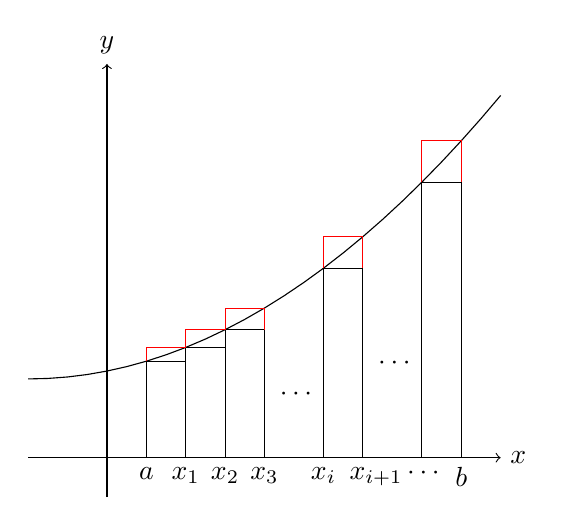
\begin{tikzpicture}
    \draw [->] (-1, 0) -- (5, 0) node [right] {$x$};
    \draw [->] (0, -0.5) -- (0, 5) node [above] {$y$};

    \draw [domain=-1:5] plot (\x, {(\x + 1)*(\x + 1)/10 + 1});

    \draw (0.5, 0) node [below] {$a$} -- (0.5, 1.225) -- (1, 1.225);
    \draw (1, 0) node [below] {$x_1$} -- (1, 1.4) -- (1.5, 1.4);
    \draw (1.5, 0) node [below] {$x_2$} -- (1.5, 1.625) -- (2, 1.625) -- (2, 0) node [below] {$x_3$};
    \node at (2.4, 0.8) {$\cdots$};
    \draw (2.75, 0) node [below] {$x_i$} -- (2.75, 2.40625) -- (3.25, 2.40625) -- (3.25, 0) node [anchor = north west] {$\!\!\!\!\!x_{i + 1}\cdots$};
    \node at (3.65, 1.2) {$\cdots$};
    \draw (4, 0) -- (4, 3.5) -- (4.5, 3.5) -- (4.5, 0) node [below] {$b$};

    \draw [red] (0.5, 1.225) -- (0.5, 1.4) -- (1, 1.4) -- (1, 1.625) -- (1.5, 1.625) -- (1.5, 1.9) -- (2, 1.9) -- (2, 1.625);
    \draw [red] (2.75, 2.40625) -- (2.75, 2.80625) -- (3.25, 2.80625) -- (3.25, 2.40625);
    \draw [red] (4, 3.5) -- (4, 4.025) -- (4.5, 4.025) -- (4.5, 3.5);
  \end{tikzpicture}
\end{center}

\begin{defi}[Refining dissections]
  If $\mathcal{D}_1$ and $\mathcal{D}_2$ are dissections of $[a, b]$, we say that $\mathcal{D}_2$ refines $\mathcal{D}_1$ if every point of $\mathcal{D}_1$ is a point of $\mathcal{D}_2$.
\end{defi}

\begin{lemma}
  If $\mathcal{D}_2$ refines $\mathcal{D}_1$, then
  \[
    U_{\mathcal{D}_2} f \leq U_{\mathcal{D}_1}f\text{ and }L_{\mathcal{D}_2 f}\geq L_{\mathcal{D}_1}f.
  \]
\end{lemma}
Using the picture above, this is because if we cut up the dissections into smaller pieces, the red rectangles can only get chopped into shorter pieces and the black rectangles can only get chopped into taller pieces.
\begin{center}
  \begin{tikzpicture}
    \draw [->] (-0.5, 0) -- (3, 0) node [right] {$x$};
    \draw [->] (0, -0.5) -- (0, 3) node [above] {$y$};

    \draw [domain=-0.5:3] plot (\x, {(\x + 1)*(\x + 1)/10 + 1});

    \draw (0.5, 0) node [below] {$x_0$} -- (0.5, 1.225) -- (2, 1.225) -- (2, 0) node [below] {$x_1$};

    \draw [red] (0.5, 1.225) -- (0.5, 1.9) -- (2, 1.9) -- (2, 1.225);
    \draw [->] (3.5, 1.5) -- (4.5, 1.5);
    \begin{scope}[shift={(5.5, 0)}]
      \draw [->] (-0.5, 0) -- (3, 0) node [right] {$x$};
      \draw [->] (0, -0.5) -- (0, 3) node [above] {$y$};

      \draw [domain=-0.5:3] plot (\x, {(\x + 1)*(\x + 1)/10 + 1});

      \draw (0.5, 0) node [below] {$x_0$} -- (0.5, 1.225) -- (1, 1.225);
      \draw (1, 0) node [below] {$x_1$} -- (1, 1.4) -- (1.5, 1.4);
      \draw (1.5, 0) node [below] {$x_2$} -- (1.5, 1.625) -- (2, 1.625) -- (2, 0) node [below] {$x_3$};

      \draw [red] (0.5, 1.225) -- (0.5, 1.4) -- (1, 1.4) -- (1, 1.625) -- (1.5, 1.625) -- (1.5, 1.9) -- (2, 1.9) -- (2, 1.625);

    \end{scope}
  \end{tikzpicture}
\end{center}

\begin{proof}
  Let $\mathcal{D}$ be $x_0 < x_1 < \cdots < x_n$. Let $\mathcal{D}_2$ be obtained from $\mathcal{D}_1$ by the addition of one point $z$. If $z\in (x_{i - 1}, x_i)$, then
  \begin{align*}
    U_{\mathcal{D}_2}f - U_{\mathcal{D}_1}f &= \left[(z - x_{i - 1}) \sup_{x\in [x_{i - 1}, z]} f(x)\right]\\
    &+ \left[(x_i - z)\sup_ {x\in[z, x_i]}f(x)\right] - (x_i - x_{i - 1})M_i.
  \end{align*}
  But $\sup_{x\in [x_{i - 1}, z]} f(x)$ and $\sup_{x\in [z, x_i]} f(x)$ are both at most $M_i$. So this is at most $M_i( z - x_{i - 1} + x_i - z - (x_i - x_{i - 1})) =0 $. So
  \[
    U_{\mathcal{D}_2} f\leq U_{\mathcal{D}_1}f.
  \]
  By induction, the result is true whenever $\mathcal{D}_2$ refines $\mathcal{D}_1$.

  A very similar argument shows that $L_{\mathcal{D}_2f} \geq L_{\mathcal{D}_1}f$.
\end{proof}
\begin{defi}[Least common refinement]
  If $\mathcal{D}_1$ and $\mathcal{D}_2$ be dissections of $[a, b]$. Then the least common refinement of $\mathcal{D}_1$ and $\mathcal{D}_2$ is the dissection made out of the points of $\mathcal{D}_1$ and $\mathcal{D}_2$.
\end{defi}

\begin{cor}
  Let $\mathcal{D}_1$ and $\mathcal{D}_2$ be two dissections of $[a, b]$. Then
  \[
    U_{\mathcal{D}_1}f \geq L_{\mathcal{D}_2}f.
  \]
\end{cor}
\begin{proof}
  Let $\mathcal{D}$ be the least common refinement (or indeed any common refinement). Then by lemma above (and by definition),
  \[
    U_{\mathcal{D}_1}f \geq U_{\mathcal{D}}f \geq L_{\mathcal{D}}f \geq L_{\mathcal{D}_2}f.\qedhere
  \]
\end{proof}

Finally, we can define the integral.
\begin{defi}[Upper, lower, and Riemann integral]
  The \emph{upper integral} is
  \[
    \overline{\int_a^b} f(x)\;\d x = \inf_{\mathcal{D}}U_{\mathcal{D}}f.
  \]
  The \emph{lower integral} is
  \[
    \underline{\int_a^b} f(x)\;\d x = \sup_{\mathcal{D}}L_{\mathcal{D}}f.
  \]
  If these are equal, then we call their common value the \emph{Riemann integral} of $f$, and is denoted $\int_a^b f(x)\;\d x$.

  If this exists, we say $f$ is \emph{Riemann integrable}.
\end{defi}
We will later prove the \emph{fundamental theorem of calculus}, which says that integration is the reverse of differentiation. But why don't we simply define integration as anti-differentiation, and prove that it is the area of the curve? There are things that we cannot find (a closed form of) the anti-derivative of, like $e^{-x^2}$. In these cases, we wouldn't want to say the integral doesn't exist --- it surely does according to this definition!

There is an immediate necessary condition for Riemann integrability --- boundedness. If $f$ is unbounded above in $[a, b]$, then for any dissection $\mathcal{D}$, there must be some $i$ such that $f$ is unbounded on $[x_{i - 1}, x_i]$. So $M_i = \infty$. So $U_\mathcal{D} f = \infty$. Similarly, if $f$ is unbounded below, then $L_{\mathcal{D}} f = -\infty$. So unbounded functions are not Riemann integrable.

\begin{eg}
  Let $f(x) = x$ on $[a, b]$. Intuitively, we know that the integral is $(b^2 - a^2)/2$, and we will show this using the definition above. Let $\mathcal{D} = x_0 < x_1 < \cdots < x_n$ be a dissection. Then
  \begin{align*}
    U_{\mathcal{D}}f &= \sum_{i = 1}^n (x_i - x_{i - 1})x_i\\
    \intertext{We \emph{know} that the integral is $\frac{b^2 - a^2}{2}$. So we put each term of the sum into the form $\frac{x_i^2 - x_{i - 1}^2}{2}$ plus some error terms.}
    &= \sum_{i = 1}^n \left(\frac{x_i^2}{2} - \frac{x_{i - 1}^2}{2} + \frac{x_i^2}{2} - x_{i - 1}x_i + \frac{x_{i - 1}^2}{2}\right)\\
    &= \frac{1}{2}\sum_{i = 1}^n (x_i^2 - x_{i - 1}^2 + (x_i - x_{i - 1})^2)\\
    &= \frac{1}{2}(b^2 - a^2) + \frac{1}{2}\sum_{i = 1}^n(x_i - x_{i - 1})^2.
  \end{align*}
  \begin{defi}[Mesh]
    The \emph{mesh} of a dissection $\mathcal{D}$ is $\max_i (x_{i+1} - x_i)$.
  \end{defi}
  Then if the mesh is $ < \delta$, then
    \[
      \frac{1}{2}\sum_{i = 1}^n (x_i - x_{i - 1})^2 \leq \frac{\delta}{2}\sum_{i = 1}^n (x_i - x_{i - 1}) = \frac{\delta}{2}(b - a).
    \]
  So by making $\delta$ small enough, we can show that for any $\varepsilon > 0$,
  \[
    \overline{\int_a^b} x\;\d x < \frac{1}{2}(b^2 - a^2) + \varepsilon.
  \]
  Similarly,
  \[
    \underline{\int_a^b} x\;\d x > \frac{1}{2}(b^2 - a^2) - \varepsilon.
  \]
  So
  \[
    \int_a^b x\;\d x = \frac{1}{2}(b^2 - a^2).
  \]
\end{eg}

\begin{eg}
  Define $f: [0, 1] \to \R$ by
  \[
    f(x) =
    \begin{cases}
      1 & x \in \Q\\
      0 & x \not\in \Q
    \end{cases}.
  \]
  Let $x_0 < x_1 < \cdots < x_n$ be a dissection. Then for every $i$, we have $m_i = 0$ (since there is an irrational in every interval), and $M_i = 1$ (since there is a rational in every interval). So
  \[
    U_{\mathcal{D}}f = \sum_{i = 1}^nM_i(x_i - x_{i - 1}) = \sum_{i = 1}^n (x_i - x_{i - 1}) = 1.
  \]
  Similarly, $L_\mathcal{D} f = 0$. Since $\mathcal{D}$ was arbitrary, we have
  \[
    \overline{\int_0^1}f(x)\;\d x = 1, \quad \underline{\int_0^1}f(x)\;\d x = 0.
  \]
  So $f$ is \emph{not} Riemann integrable.

  Of course, this function is not interesting at all. The whole point of its existence is to show undergraduates that there are some functions that are not integrable!
\end{eg}

Note that it is important to say that the function is not \emph{Riemann} integrable. There are other notions for integration in which this function is integrable. For example, this function is \emph{Lebesgue-integrable}.

Using the definition to show integrability is often cumbersome. Most of the time, we use the \emph{Riemann's integrability criterion}, which follows rather immediately from the definition, but is much nicer to work with.
\begin{prop}[Riemann's integrability criterion]
  This is sometimes known as Cauchy's integrability criterion.

  Let $f: [a, b] \to \R$. Then $f$ is Riemann integrable if and only if for every $\varepsilon > 0$, there exists a dissection $\mathcal{D}$ such that
  \[
    U_\mathcal{D} - L_\mathcal{D} < \varepsilon.
  \]
\end{prop}

\begin{proof}
  $(\Rightarrow)$ Suppose that $f$ is integrable. Then (by definition of Riemann integrability), there exist $\mathcal{D}_1$ and $\mathcal{D}_2$ such that
  \[
    U_{\mathcal{D}_1} < \int_a^b f(x)\;\d x + \frac{\varepsilon}{2},
  \]
  and
  \[
    L_{\mathcal{D}_2} > \int_a^b f(x)\;\d x - \frac{\varepsilon}{2}.
  \]
  Let $\mathcal{D}$ be a common refinement of $\mathcal{D}_1$ and $\mathcal{D}_2$. Then
  \[
    U_\mathcal{D} f - L_\mathcal{D} f \leq U_{\mathcal{D}_1} f- L_{\mathcal{D}_2} f < \varepsilon.
  \]
  $(\Leftarrow)$ Conversely, if there exists $\mathcal{D}$ such that
  \[
    U_\mathcal{D} f - L_\mathcal{D}f < \varepsilon,
  \]
  then
  \[
    \inf U_\mathcal{D} f - \sup L_\mathcal{D} f < \varepsilon,
  \]
  which is, by definition, that
  \[
    \overline{\int_a^b} f(x)\;\d x - \underline{\int_a^b} f(x)\;\d x < \varepsilon.
  \]
  Since $\varepsilon > 0$ is arbitrary, this gives us that
  \[
    \overline{\int_a^b} f(x)\;\d x = \underline{\int_a^b} f(x)\;\d x.
  \]
  So $f$ is integrable.
\end{proof}

The next big result we want to prove is that integration is linear, ie
\[
  \int_a^b (\lambda f(x) + \mu g(x))\;\d x = \lambda\int_a^b f(x)\;\d x + \mu\int_a^bg(x)\;\d x.
\]
We do this step by step:
\begin{prop}
  Let $f: [a, b] \to \R$ be integrable, and $\lambda \geq 0$. Then $\lambda f$ is integrable, and
  \[
    \int_a^b \lambda f(x)\;\d x = \lambda\int_a^b f(x)\;\d x.
  \]
\end{prop}

\begin{proof}
  Let $\mathcal{D}$ be a dissection of $[a, b]$. Since
  \[
    \sup_{x\in [x_{i - 1}, x_i]}\lambda f(x) = \lambda\sup_{x\in [x_{i - 1}, x_i]}f(x),
  \]
  and similarly for inf, we have
  \begin{align*}
    U_{\mathcal{D}}(\lambda f) &= \lambda U_{\mathcal{D}} f\\
    L_{\mathcal{D}}(\lambda f) &= \lambda L_\mathcal{D} f.
  \end{align*}
  So if we choose $\mathcal{D}$ such that $U_{\mathcal{D}}f - L_\mathcal{D} f < \varepsilon/\lambda$, then $U_\mathcal{D}(\lambda f) - L_\mathcal{D}(\lambda f) < \varepsilon$. So the result follows from Riemann's integrability criterion.
\end{proof}

\begin{prop}
  Let $f: [a, b] \to \R$ be integrable. Then $-f$ is integrable, and
  \[
    \int_a^b -f(x)\;\d x = -\int_a^bf(x)\;\d x.
  \]
\end{prop}

\begin{proof}
  Let $\mathcal{D}$ be a dissection. Then
  \begin{align*}
    \sup_{x\in [x_{i - 1}, x_i]}-f(x) &= -\inf_{x\in [x_{i - 1}, x_i]} f(x)\\
    \inf_{x\in [x_{i - 1}, x_i]}-f(x) &= -\sup_{x\in [x_{i - 1}, x_i]} f(x).
  \end{align*}
  Therefore
  \[
    U_\mathcal{D}(-f) = \sum_{i = 1}^n (x_i - x_{i - 1})(-m_i) = -L_\mathcal{D}(f).
  \]
  Similarly,
  \[
    L_\mathcal{D}(-f) = -U_\mathcal{D}f.
  \]
  So
  \[
    U_\mathcal{D}(-f) - L_\mathcal{D}(-f) = U_\mathcal{D}f - L_\mathcal{D}f.
  \]
  Hence if $f$ is integrable, then $-f$ is integrable by the Riemann integrability criterion.
\end{proof}

\begin{prop}
  Let $f, g: [a, b] \to \R$ be integrable. Then $f + g$ is integrable, and
  \[
    \int_a^b(f(x) + g(x))\;\d x = \int_a^b f(x)\;\d x + \int_a^b g(x)\;\d x.
  \]
\end{prop}

\begin{proof}
  Let $\mathcal{D}$ be a dissection. Then
  \begin{align*}
    U_\mathcal{D}(f + g) &= \sum_{i = 1}^n (x_i - x_{i - 1})\sup_{x\in [x_{i - 1}, x_i]}(f(x) + g(x))\\
    &\leq \sum_{i = 1}^n (x_i - x_{i - 1}) \left(\sup_{u\in [x_{i - 1}, x_i]}f(u) + \sup_{v\in [x_{i - 1}, x_i]}g(v)\right)\\
    &= U_\mathcal{D}f + U_\mathcal{D} g
  \end{align*}
  Therefore,
  \[
    \overline{\int_a^b}(f(x) + g(x))\;\d x \leq \overline{\int_a^b} f(x)\;\d x + \overline{\int_a^b} g(x)\;\d x = \int_a^b f(x)\;\d x + \int_a^bg(x)\;\d x.
  \]
  Similarly,
  \[
  \underline{\int_a^b}(f(x) + g(x))\;\d x \geq \int_a^b f(x)\;\d x + \int_a^b g(x)\;\d x.
  \]
  So the upper and lower integrals are equal, and the result follows.
\end{proof}
So we now have that
\[
  \int_a^b (\lambda f(x) + \mu g(x))\;\d x = \lambda\int_a^b f(x)\;\d x + \mu\int_a^bg(x)\;\d x.
\]
We will prove more ``obvious'' results.
\begin{prop}
  Let $f, g: [a, b] \to \R$ be integrable, and suppose that $f(x) \leq g(x)$ for every $x$. Then
  \[
    \int_a^b f(x)\;\d x \leq \int_a^b g(x)\;\d x.
  \]
\end{prop}

\begin{proof}
  Follows immediately from the definition.
\end{proof}

\begin{prop}
  Let $f: [a, b] \to \R$ be integrable. Then $|f|$ is integrable.
\end{prop}

\begin{proof}
  Note that we can write
  \[
    \sup_{x\in [x_{i - 1}, x_i]}f(x) - \inf_{x\in [x_{i - 1}, x_i]}f(x) = \sup_{u, v\in [x_{i - 1}, x_i]}|f(u) - f(v)|.
  \]
  Similarly,
  \[
    \sup_{x\in [x_{i - 1}, x_i]}|f(x)| - \inf_{x\in [x_{i - 1}, x_i]}|f(x)| = \sup_{u, v\in [x_{i - 1}, x_i]}||f(u)| - |f(v)||.
  \]
  For any pair of real numbers, $x, y$, we have that $||x| - |y|| \leq |x - y|$ by the triangle inequality. Then for any interval $u, v\in [x_{i - 1}, x_i]$, we have
  \[
    ||f(u)| - |f(v)|| \leq |f(u) - f(v)|.
  \]
  Hence we have
  \[
    \sup_{x\in [x_{i - 1}, x_i]}|f(x)| - \inf_{x\in [x_{i - 1}, x_i]}|f(x)| \leq \sup_{x\in [x_{i - 1}, x_i]}f(x) - \inf_{x\in [x_{i - 1}, x_i]} f(x).
  \]
  So for any dissection $\mathcal{D}$, we have
  \[
    U_\mathcal{D} (|f|) - L_\mathcal{D}(|f|) \leq U_\mathcal{D}(f) - L_\mathcal{D}(f).
  \]
  So the result follows from Riemann's integrability criterion.
\end{proof}
Combining these two propositions, we get that if
\[
  |f(x) - g(x)| \leq C,
\]
for every $x\in[a, b]$, then
\[
  \left|\int_a^bf(x)\;\d x - \int_a^b g(x)\;\d x\right| \leq C(b - a).
\]

\begin{prop}[Additivity property]
  Let $f: [a, c] \to \R$ be integrable, and let $b\in (a, c)$. Then the restrictions of $f$ to $[a, b]$ and $[b, c]$ are Riemann integrable, and
  \[
    \int_a^b f(x)\;\d x + \int_b^c f(x)\;\d x = \int_a^c f(x) \;\d x
  \]
  Similarly, if $f$ is integrable on $[a, b]$ and $[b, c]$, then it is integrable on $[a, c]$ and the above equation also holds.
\end{prop}

\begin{proof}
  Let $\varepsilon> 0$, and let $a = x_0 < x_1 < \cdots < x_n = c$ be a dissection of $\mathcal{D}$ of $[a, c]$ such that
  \[
    U_\mathcal{D}(f) \leq \int_a^c f(x)\;\d x + \varepsilon,
  \]
  and
  \[
    L_\mathcal{D}(f) \geq \int_a^c f(x)\;\d x - \varepsilon.
  \]
  Let $\mathcal{D}'$ be the dissection made of $\mathcal{D}$ plus the point $b$. Let $\mathcal{D}_1$ be the dissection of $[a, b]$ made of points of $\mathcal{D}'$ from $a$ to $b$, and $D_2$ be the dissection of $[b, c]$ made of points of $\mathcal{D}'$ from $b$ to $c$. Then
  \[
    U_{\mathcal{D}_1}(f) + U_{\mathcal{D}_2}(f) = U_{\mathcal{D}'}(f) \leq U_{\mathcal{D}}(f),
  \]
  and
  \[
    L_{\mathcal{D}_1}(f) + L_{\mathcal{D}_2}(f) = L_{\mathcal{D}'}(f) \geq L_\mathcal{D} (f).
  \]
  Since $U_\mathcal{D}(f) - L_\mathcal{D}(f) < 2\varepsilon$, and both $U_{\mathcal{D}_2}(f) - L_{\mathcal{D}_2} (f)$ and $U_{\mathcal{D}_1}(f) - L_{\mathcal{D}_1} (f)$ are non-negative, we have $U_{\mathcal{D}_1} (f) - L_{\mathcal{D}_1} (f)$ and $U_{\mathcal{D}_2}(f) - L_{\mathcal{D}_2}(f)$ are less than $2\varepsilon$. Since $\varepsilon$ is arbitrary, it follows that the restrictions of $f$ to $[a, b]$ and $[b, c]$ are both Riemann integrable. Furthermore,
  \begin{multline*}
    \int_a^b f(x)\;\d x + \int_b^c f(x)\;\d x \leq U_{\mathcal{D}_1}(f) + U_{\mathcal{D}_2}(f) = U_{\mathcal{D}'}(f) \leq U_{\mathcal{D}}(f)\\
    \leq \int_a^c f(x)\;\d x + \varepsilon.
  \end{multline*}
  Similarly,
  \begin{multline*}
    \int_a^bf(x)\;\d x + \int_b^cf(x)\;\d x \geq L_{\mathcal{D}_1}(f) + L_{\mathcal{D}_2}(f) = L_{\mathcal{D}'}(f) \geq L_{\mathcal{D}}(f)\\
    \geq \int_a^c f(x)\;\d x - \varepsilon.
  \end{multline*}
  Since $\varepsilon$ is arbitrary, it follows that
  \[
    \int_a^b f(x)\;\d x + \int_b^c f(x)\;\d x = \int_a^c f(x)\;\d x.
  \]
  The other direction is left as an (easy) exercise.
\end{proof}

\begin{prop}
  Let $f, g: [a, b] \to \R$ be integrable. Then $fg$ is integrable.
\end{prop}

\begin{proof}
  Let $C$ be such that $|f(x)|, |g(x)| \leq C$ for every $x\in [a, b]$. Write $L_i$ and $\ell_i$ for the $\sup$ and $\inf$ of $g$ in $[x_{i - 1}, x_i]$. Now let $\mathcal{D}$ be a dissection, and for each $i$, let $u_i$ and $v_i$ be two points in $[x_{i - 1}, x_i]$.

  We will pretend that $u_i$ and $v_i$ are the maximum and minimum when we write the proof, but we cannot assert that they are, since $fg$ need not have maxima and minima. We will then note that since our results hold for arbitrary $u_i$ and $v_i$, it must hold when $fg$ is at its supremum and infimum.

  We find what we pretend is the difference between the upper and lower sum:
  \begin{align*}
    &\quad \left|\sum_{i = 1}^n \big(x_i - x_{i - 1})(f(v_i)g(v_i) - f(u_i)g(u_i)\big)\right| \\
    &= \left|\sum_{i = 1}^{n}(x_i - x_{i - 1})\big(f(v_i)(g(v_i) - g(u_i)) + (f(v_i - f(u_i))g(u_i))\big)\right|\\
    &\leq \sum_{i = 1}^n \big(C(L_i - \ell_i) + (M_i - m_i)C\big)\\
    &=C(U_\mathcal{D}g - L_\mathcal{D}g + U_\mathcal{D}f - L_\mathcal{D}f).
  \end{align*}
  Since $u_i$ and $v_i$ are arbitrary, it follows that
  \[
    U_\mathcal{D}(fg) - L_\mathcal{D}(fg) \leq C(U_\mathcal{D}f - L_\mathcal{D}f + U_\mathcal{D}g - L_\mathcal{D}g).
  \]
  Since $C$ is fixed, and we can get $U_\mathcal{D} f - L_\mathcal{D}f$ and $U_\mathcal{D}g - L_\mathcal{D}g$ arbitrary small (since $f$ and $g$ are integrable), we can get $U_\mathcal{D}(fg) - L_\mathcal{D}(fg)$ arbitrarily small. So the result follows.
\end{proof}

\begin{thm}
  Every continuous function $f$ on a closed bounded interval $[a, b]$ is Riemann integrable.
\end{thm}

\begin{proof}
  wlog assume $[a, b] = [0, 1]$.

  Suppose the contrary. Let $f$ be non-integrable. This means that there exists some $\varepsilon$ such that for every dissection $\mathcal{D}$, $U_{\mathcal{D}} - L_{\mathcal{D}} > \varepsilon$. In particular, for every $n$, let $\mathcal{D}_n$ be the dissection $0, \frac{1}{n}, \frac{2}{n}, \cdots, \frac{n}{n}$.

  Since $U_{\mathcal{D}_n} - L_{\mathcal{D}_n} > \varepsilon$, there exists some interval $\left[\frac{k}{n}, \frac{k + 1}{n}\right]$ in which $\sup f - \inf f > \varepsilon$. Suppose the supremum and infimum are attained at $x_n$ and $y_n$ respectively. Then we have $|x_n - y_n| < \frac{1}{n}$ and $f(x_n) - f(y_n) > \varepsilon$.

  By Bolzano Weierstrass, $(x_n)$ has a convergent subsequence, say $(x_{n_i})$. Say $x_{n_i}\to x$. Since $|x_n - y_n| < \frac{1}{n}\to 0$, we must have $y_{n_i}\to x$. By continuity, we must have $f(x_{n_i}) \to f(x)$ and $f(y_{n_i}) \to f(x)$, but $f(x_{n_i})$ and $f(y_{n_i})$ are always apart by $\varepsilon$. Contradiction.
\end{proof}
With this result, we know that a lot of things are integrable, e.g.\ $e^{-x^2}$.

To prove this, we secretly used the property of \emph{uniform continuity}:
\begin{defi}[Uniform continuity*]
  Let $A\subseteq \R$ and let $f: A\to \R$. Then $f$ is \emph{uniformly continuous} if
  \[
    (\forall \varepsilon)(\exists \delta > 0)(\forall x)(\forall y)\;|x - y| < \delta \Rightarrow |f(x) - f(y)| \leq \varepsilon.
  \]
\end{defi}
This is different from regular continuity. Regular continuity says that at any point $x$, we can find a $\delta$ that works for this point. Uniform continuity says that we can find a $\delta$ that works for \emph{any} $x$.

It is easy to show that a uniformly continuous function is integrable, since by uniformly continuity, as long as the mesh of a dissection is sufficiently small, the difference between the upper sum and the lower sum can be arbitrarily small by uniform continuity. Thus to prove the above theorem, we just have to show that continuous functions on a closed bounded interval are uniformly continuous.

\begin{thm}[non-examinable]
  Let $a < b$ and let $f: [a, b] \to \R$ be continuous. Then $f$ is uniformly continuous.
\end{thm}

\begin{proof}
  Suppose that $f$ is not uniformly continuous. Then
  \[
    (\exists \varepsilon)(\forall \delta > 0)(\exists x)(\exists y)\;|x - y| < \delta \text{ and } |f(x) - f(y)| \geq \varepsilon.
  \]
  Therefore, we can find sequences $(x_n), (y_n)$ such that for every $n$, we have
  \[
    |x_n - y_n| \leq \frac{1}{n}\text{ and }|f(x_n) - f(y_n)| \geq \varepsilon.
  \]
  Then by Bolzano-Weierstrass theorem, we can find a subsequence $(x_{n_k})$ converging to some $x$. Since $|x_{n_k} - y_{n_k}| \leq \frac{1}{n_k}$, $y_{n_k}\to x$ as well. But $|f(x_{n_k}) - f(y_{n_k})| \geq \varepsilon$ for every $k$. So $f(x_{n_k})$ and $f(y_{n_k})$ cannot both converge to the same limit. So $f$ is not continuous at $x$.
\end{proof}
This proof is very similar to the proof that continuous functions are integrable. In fact, the proof that continuous functions are integrable is just a fuse of this proof and the (simple) proof that uniformly continuously functions are integrable.

\begin{thm}
  Let $f: [a, b] \to \R$ be monotone. Then $f$ is Riemann integrable.
\end{thm}
Note that monotone functions need not be ``nice''. It can even have infinitely many discontinuities. For example, if $f: [0, 1] \to \R$ maps $x$ to the $1/(\text{first non-zero digit in the binary expansion of }x)$, with $f(0) = 0$.

\begin{proof}
  let $\varepsilon > 0$. Let $\mathcal{D}$ be a dissection of mesh less than $\frac{\varepsilon}{f(b) - f(a)}$. Then
  \begin{align*}
    U_\mathcal{D} f - L_\mathcal{D}f &= \sum_{i = 1}^n (x_i - x_{i - 1})(f(x_i) - f(x_{i - 1}))\\
    &\leq \frac{\varepsilon}{f(b) - f(a)} \sum_{i = 1}^n (f(x_i) - f(x_{i - 1}))\\
    &= \varepsilon.\qedhere
  \end{align*}
\end{proof}

Pictorially, we see that the difference between the upper and lower sums is total the area of the red rectangles.
\begin{center}
  \begin{tikzpicture}
    \draw [->] (-1, 0) -- (5, 0) node [right] {$x$};
    \draw [->] (0, -0.5) -- (0, 5) node [above] {$y$};

    \draw [domain=-1:5] plot (\x, {(\x + 1)*(\x + 1)/10 + 1});

    \draw (0.5, 0) rectangle (1, 1.225);
    \draw (1, 0) rectangle (1.5, 1.4);
    \draw (1.5, 0) rectangle (2, 1.625);
    \draw (2, 0) rectangle (2.5, 1.9);
    \draw (2.5, 0) rectangle (3, 2.225);
    \draw (3, 0) rectangle (3.5, 2.6);
    \draw (3.5, 0) rectangle (4, 3.026);
    \draw (4, 0) rectangle (4.5, 3.5);

    \draw [red] (0.5, 1.225) rectangle (1, 1.4);
    \draw [red] (1, 1.4) rectangle (1.5, 1.625);
    \draw [red] (1.5, 1.625) rectangle (2, 1.9);
    \draw [red] (2, 1.9) rectangle (2.5, 2.225);
    \draw [red] (2.5, 2.225) rectangle (3, 2.6);
    \draw [red] (3, 2.6) rectangle (3.5, 3.025);
    \draw [red] (3.5, 3.025) rectangle (4, 3.5);
    \draw [red] (4, 3.5) rectangle (4.5, 4.025);
  \end{tikzpicture}
\end{center}
To calculate the total area, we can stack the red areas together to get something of width $\frac{\varepsilon}{f(b) - f(a)}$ and height $f(b) - f(a)$. So the total area is just $\varepsilon$.

\begin{lemma}
  Let $a < b$ and let $f$ be a bounded function from $[a, b] \to \R$ that is continuous on $(a, b)$. Then $f$ is integrable.
\end{lemma}
An example where this would apply is $\int_0^1 \sin \frac{1}{x}$. It gets nasty near $x = 0$, but its ``nastiness'' is confined to $x = 0$ only. So as long as its nastiness is sufficiently contained, it would still be integrable.

The idea of the proof is to integrate from a point $x_1$ very near $a$ up to a point $x_{n - 1}$ very close to $b$. Since $f$ is bounded, the regions $[a, x_1]$ and $[x_{n - 1}, b]$ are small enough to not cause trouble.

\begin{proof}
  Let $\varepsilon > 0$. Suppose that $|f(x)| \leq C$ for every $x\in [a, b]$. Let $x_0 = a$ and pick $x_1$ such that $x_1 - x_0 < \frac{\varepsilon}{8C}$. Also choose $z$ between $x_1$ and $b$ such that $b - z < \frac{\varepsilon}{8C}$.

  Then $f$ is continuous $[x_1, z]$. Therefore it is integrable on $[x_1, z]$. So we can find a dissection $\mathcal{D}'$ with points $x_1 < x_2 < \cdots < x_{n - 1} = z$ such that
  \[
    U_{\mathcal{D}'}f - L_{\mathcal{D}'}f < \frac{\varepsilon}{2}.
  \]
  Let $\mathcal{D}$ be the dissection $a = x_0 < x_1 < \cdots < x_n = b$. Then
  \[
    U_\mathcal{D} f - L_\mathcal{D} f < \frac{\varepsilon}{8C}\cdot 2C + \frac{\varepsilon}{2} + \frac{\varepsilon}{8C}\cdot 2C = \varepsilon.
  \]
  So done by Riemann integrability criterion.
\end{proof}

\begin{eg}\leavevmode
  \begin{itemize}
    \item $f(x) =
      \begin{cases}
        \sin \frac{1}{x}& x \not = 0\\
        0 & x = 0
      \end{cases}$ defined on $[-1, 1]$ is integrable.
    \item $g(x) =
      \begin{cases}
        x & x \leq 1\\
        x^2 + 1 & x > 1
      \end{cases}$ defined on $[0, 1]$ is integrable.
  \end{itemize}
\end{eg}

\begin{cor}
  Every piecewise continuous and bounded function on $[a, b]$ is integrable.
\end{cor}

\begin{proof}
  Partition $[a, b]$ into intervals $I_1, \cdots, I_k$, on each of which $f$ is (bounded and) continuous. Hence for every $I_j$ with end points $x_{j - 1}$, $x_j$, $f$ is integrable on $[x_{j - 1}, x_j]$ (which may not equal $I_j$, e.g.\ $I_j$ could be $[x_{j - 1}, x_j)$). But then by the additivity property of integration, we get that $f$ is integrable on $[a, b]$
\end{proof}

We defined Riemann integration in a very general way --- we allowed \emph{arbitrary} dissections, and took the extrema over all possible dissection. Is it possible to just consider some particular nice dissections instead? Perhaps unsurprisingly, yes! It's just that we opt to define it the general way so that we can easily talk about things like least common refinements.
\begin{lemma}
  Let $f: [a, b] \to \R$ be Riemann integrable, and for each $n$, let $\mathcal{D}_n$ be the dissection $a = x_0 < x_1 < \cdots < x_n = b$, where $x_i = a + \frac{i(b - a)}{n}$ for each $i$. Then
  \[
    U_{\mathcal{D}_n}f \to \int_a^b f(x)\;\d x
  \]
  and
  \[
    L_{\mathcal{D}_n}f \to \int_a^b f(x)\;\d x.
  \]
\end{lemma}

\begin{proof}
  Let $\varepsilon > 0$. We need to find an $N$. The only thing we know is that $f$ is Riemann integrable, so we use it:

  Since $f$ is integrable, there is a dissection $\mathcal{D}$, say $u_0 < u_1 < \cdots < u_m$, such that
  \[
    U_\mathcal{D} f - \int_a^b f(x)\;\d x < \frac{\varepsilon}{2}.
  \]
  We also know that $f$ is bounded. Let $C$ be such that $|f(x)| \leq C$.

  For any $n$, let $\mathcal{D}'$ be the least common refinement of $\mathcal{D}_n$ and $\mathcal{D}$. Then
  \[
    U_{\mathcal{D}'}f \leq U_\mathcal{D} f.
  \]
  Also, the sums $U_{\mathcal{D}_n}f$ and $U_\mathcal{D'}f$ are the same, except that at most $m$ of the subintervals $[x_{i - 1}, x_i]$ are subdivided in $\mathcal{D}'$.

  For each interval that gets chopped up, the upper sum decreases by at most $\frac{b - a}{n}\cdot 2C$. Therefore
  \[
    U_{\mathcal{D}_n}f - U_{\mathcal{D}'}f \leq \frac{b - a}{n}2C\cdot m.
  \]
  Pick $n$ such that $2Cm(b - a)/n < \frac{\varepsilon}{2}$. Then
  \[
    U_{\mathcal{D}_n} f - U_\mathcal{D}f < \frac{\varepsilon}{2}.
  \]
  So
  \[
    U_{\mathcal{D}_n}f - \int_a^b f(x)\;\d x < \varepsilon.
  \]
  This is true whenever $n > \frac{4C(b - a)m}{\varepsilon}$. Since we also have $U_{\mathcal{D}_n} f \geq \int_a^b f(x)\;\d x$, therefore
  \[
    U_{\mathcal{D}_n}f \to \int_a^b f(x)\;\d x.
  \]
  The proof for lower sums is similar.
\end{proof}

For convenience, we define the following:
\begin{notation}
  If $b > a$, we define
  \[
    \int_b^a f(x)\;\d x = -\int_a^b f(x)\;\d x.
  \]
\end{notation}

We now prove that the fundamental theorem of calculus, which says that integration is the reverse of differentiation.
\begin{thm}[Fundamental theorem of calculus, part 1]
  Let $f: [a, b]\to \R$ be continuous, and for $x\in [a, b]$, define
  \[
    F(x) = \int_a^x f(t)\;\d t.
  \]
  Then $F$ is differentiable and $F'(x) = f(x)$ for every $x$.
\end{thm}

\begin{proof}
  \[
    \frac{F(x + h) - F(x)}{h} = \frac{1}{h}\int_x^{x + h}f(t)\;\d t
  \]
  Let $\varepsilon > 0$. Since $f$ is continuous, at $x$, then there exists $\delta$ such that $|y - x| < \delta$ implies $|f(y) - f(x)| < \varepsilon$.

  If $|h| < \delta$, then
  \begin{align*}
    \left|\frac{1}{h}\int_x^{x + h}f(t) \;\d t - f(x)\right| &= \left|\frac{1}{h}\int_x^{x + h}(f(t) - f(x))\;\d t\right|\\
    &\leq \frac{1}{|h|}\left|\int_x^{x + h}|f(t) - f(x)|\;\d t\right|\\
    &\leq \frac{\varepsilon|h|}{|h|}\\
    &= \varepsilon.\qedhere
  \end{align*}
\end{proof}

\begin{cor}
  If $f$ is continuously differentiable on $[a, b]$, then
  \[
    \int_a^b f'(t)\;\d t = f(b) - f(a).
  \]
\end{cor}

\begin{proof}
  Let
  \[
    g(x) = \int_a^x f'(t)\;\d t.
  \]
  Then
  \[
    g'(x) = f'(x) = \frac{\d }{\d x}(f(x) - f(a)).
  \]
  Since $g'(x) - f'(x) = 0$, $g(x) - f(x)$ must be a constant function by the mean value theorem. We also know that
  \[
    g(a) = 0 = f(a) - f(a)
  \]
  So we must have $g(x) = f(x) - f(a)$ for every $x$, and in particular, for $x = b$.
\end{proof}

\begin{thm}[Fundamental theorem of calculus, part 2]
  Let $f: [a, b] \to \R$ be a differentiable function, and suppose that $f'$ is integrable. Then
  \[
    \int_a^b f'(t)\;\d t = f(b) - f(a).
  \]
\end{thm}
Note that this is a stronger result than the corollary above, since it does not require that $f'$ is continuous.

\begin{proof}
  Let $\mathcal{D}$ be a dissection $x_0 < x_1 < \cdots < x_n$. We want to make use of this dissection. So write
  \[
    f(b) - f(a) = \sum_{i = 1}^n (f(x_i) - f(x_{i - 1})).
  \]
  For each $i$, there exists $u_i\in (x_{i - 1}, x_i)$ such that $f(x_i) - f(x_{i - 1j}) = (x_i - x_{i - 1})f'(u_i)$ by the mean value theorem. So
  \[
    f(b) - f(a) = \sum_{i = 1}^n (x_i - x_{i - 1})f'(u_i).
  \]
  We know that $f'(u_i)$ is somewhere between $\sup\limits_{x\in[x_i, x_{i - 1}]}f'(x)$ and $\inf\limits_{x\in[x_i, x_{i - 1}]}f'(x)$ by definition. Therefore
  \[
    L_\mathcal{D} f' \leq f(b) - f(a) \leq U_\mathcal{D} f'.
  \]
  Since $f'$ is integrable and $\mathcal{D}$ was arbitrary, $L_\mathcal{D}f'$ and $U_\mathcal{D}f'$ can both get arbitrarily close to $\int_a^b f'(t)\;\d t$. So
  \[
    f(b) - f(a) = \int_a^b f'(t)\;\d t.\qedhere
  \]
\end{proof}
Note that the condition that $f'$ is integrable is essential. It is possible to find a differentiable function whose derivative is not integrable! You will be asked to find it in the example sheet.

Using the fundamental theorem of calculus, we can easily prove integration by parts:
\begin{thm}[Integration by parts]
  Let $f, g:[a, b]\to \R$ be integrable such that everything below exists. Then
  \[
    \int_a^b f(x)g'(x)\;\d x = f(b)g(b) - f(a)g(a) - \int_a^b f'(x)g(x)\;\d x.
  \]
\end{thm}

\begin{proof}
  By the fundamental theorem of calculus,
  \[
    \int_a^b (f(x)g'(x) + f'(x)g(x))\;\d x = \int_a^b(fg)'(x)\;\d x = f(b)g(b) - f(a)g(a).
  \]
  The result follows after rearrangement.
\end{proof}

Recall that when we first had Taylor's theorem, we said it had the Lagrange form of the remainder. There are many other forms of the remainder term. Here we will look at the integral form:
\begin{thm}[Taylor's theorem with the integral form of the remainder]
  Let $f$ be $n + 1$ times differentiable on $[a, b]$ with with $f^{(n + 1)}$ continuous. Then
  \begin{align*}
    f(b) &= f(a) + (b - a)f'(a) + \frac{(b - a)^2}{2!}f^{(2)}(a) + \cdots \\
    &+ \frac{(b - a)^n}{n!}f^{(n)}(a) + \int_a^b \frac{(b - t)^n}{n!}f^{(n + 1)}(t)\;\d t.
  \end{align*}
\end{thm}
\begin{proof}
  Induction on $n$.

  When $n = 0$, the theorem says
  \[
    f(b) - f(a) = \int_a^b f'(t)\;\d t.
  \]
  which is true by the fundamental theorem of calculus.

  Now observe that
  \begin{align*}
    \int_a^b \frac{(b - t)^n}{n!}f^{(n + 1)}(t)\;\d t ={}& \left[\frac{-(b - t)^{n + 1}}{(n + 1)!}f^{(n + 1)}(t)\right]_a^b\\
    &+ \int_a^b \frac{(b - t)^{n + 1}}{(n + 1)!}f^{(n + 1)}(t)\;\d t \\
    ={}& \frac{(b - a)^{n + 1}}{(n + 1)!} f^{(n + 1)}(a) + \int_a^b \frac{(b - t)^{n + 1}}{(n + 1)!}f^{(n + 2)}(t)\;\d t.
  \end{align*}
  So the result follows by induction.
\end{proof}
Note that the form of the integral remainder is rather weird and unexpected. How could we have come up with it? We might start with the fundamental theorem of algebra and integrate by parts. The first attempt would be to integrate $1$ to $t$ and differentiate $f'(t)$ to $f^{(2)}(t)$. So we have
\begin{align*}
  f(b) &= f(a) + \int_a^b f'(t)\;\d t\\
  &= f(a) + [tf'(t)]_a^b - \int_a^b tf^{(2)}(t)\;\d t\\
  &= f(a) + bf'(b) - af'(a) - \int_a^b tf^{(2)}(t)\;\d t\\
  \intertext{We want something in the form $(b - a)f'(a)$, so we take that out and see what we are left with.}
  &= f(a) + (b - a)f'(a) + b(f'(b) - f'(a)) - \int_a^b tf^{(2)}(t)\;\d t\\
  \intertext{Then we note that $f'(b) - f'(a) = \int_a^b f^{(2)}(t)\;\d t$. So we have}
  &= f(a) + (b - a)f'(a) + \int_a^b (b - t)f^{(2)}(t)\;\d t.
\end{align*}
Then we can see that the right thing to integrate is $(b - t)$ and continue to obtain the result.

\begin{thm}[Integration by substitution]
  Let $f: [a, b] \to \R$ be continuous. Let $g: [u, v] \to \R$ be continuously differentiable, and suppose that $g(u) = a, g(v) = b$, and $f$ is defined everywhere on $g([u, v])$ (and still continuous). Then
  \[
    \int_a^b f(x)\;\d x = \int_u^v f(g(t))g'(t)\;\d t.
  \]
\end{thm}

\begin{proof}
  By the fundamental theorem of calculus, $f$ has an anti-derivative $F$ defined on $g([u, v])$. Then
  \begin{align*}
    \int_u^v f(g(t))g'(t) \;\d t &= \int_u^v F'(g(t))g'(t)\;\d t \\
    &= \int_u^v (F\circ g)'(t)\;\d t \\
    &= F\circ g(v) - F\circ g(u)\\
    &= F(b) - F(a)\\
    &= \int_a^b f(x)\;\d x.\qedhere
  \end{align*}
\end{proof}
We can think of ``integration by parts'' as what you get by integrating the product rule, and ``integration by substitution'' as what you get by integrating the chain rule.

\subsection{Improper integrals}
It is sometimes sensible to talk about integrals of unbounded functions or integrating to infinity. But we have to be careful and write things down nicely.

\begin{defi}[Improper integral]
  Suppose that we have a function $f: [a, b] \to \R$ such that, for every $\varepsilon > 0$, $f$ is integrable on $[a + \varepsilon, b]$ and $\lim\limits_{\varepsilon \to 0}\int_{a + \varepsilon}^b f(x)\;\d x$ exists. Then we define the improper integral
  \[
    \int_a^bf(x)\;\d x \text{ to be } \lim_{\varepsilon \to 0}\int_{a + \varepsilon}^b f(x)\;\d x.
  \]
  even if the Riemann integral does not exist.

  We can do similarly for $[a, b - \varepsilon]$, or integral to infinity:
  \[
    \int_a^\infty f(x)\;\d x = \lim_{b \to \infty} \int_a^b f(x)\;\d x.
  \]
  when it exists.
\end{defi}
\begin{eg}
  \[
    \int_\varepsilon^1 x^{-1/2}\;\d x = \left[2x^{-1/2}\right]^1_\varepsilon = 2 - 2\varepsilon^{1/2} \to 2.
  \]
  So
  \[
    \int_0^1 x^{-1/2}\;\d x = 2,
  \]
  even though $x^{-1/2}$ is unbounded on $[0, 1]$.

  Note that officially we are required to make $f(x) = x^{-1/2}$ a function with domain $[0, 1]$. So we can assign $f(0) = \pi$, or any number, since it doesn't matter.
\end{eg}

\begin{eg}
  \[
    \int_1^x \frac{1}{t^2}\;\d t = \left[-\frac{1}{t}\right]_1^x = 1 - \frac{1}{x} \to 1\text{ as }x\to \infty
  \]
  by the fundamental theorem of calculus. So
  \[
    \int_1^{\infty}\frac{1}{x^2}\;\d x = 1.
  \]
\end{eg}

Finally, we can prove the integral test, whose proof we omitted when we first began.
\begin{thm}[Integral test]
  Let $f: [1, \infty] \to \R$ be a decreasing non-negative function. Then $\sum_{n = 1}^\infty f(n)$ converges iff $\int_1^\infty f(x)\;\d x < \infty$.
\end{thm}

\begin{proof}
  We have
  \[
    \int_n^{n + 1}f(x)\;\d x \leq f(n) \leq \int_{n -1}^n f(x)\;\d x,
  \]
  since $f$ is decreasing (the right hand inequality is valid only for $n\geq 2$). It follows that
  \[
    \int_1^{N + 1}f(x)\;\d x \leq \sum_{n = 1}^N f(n) \leq \int_1^N f(x)\;\d x + f(1)
  \]
  So if the integral exists, then $\sum f(n)$ is increasing and bounded above by $\int_1^\infty f(x)\;\d x$, so converges.

  If the integral does not exist, then $\int_1^N f(x)\;\d x$ is unbounded. Then $\sum_{n = 1}^N f(n)$ is unbounded, hence does not converge.
\end{proof}

\begin{eg}
  Since $\int_1^x \frac{1}{t^2}\;\d t < \infty$, it follows that $\sum_{n = 1}^\infty \frac{1}{n^2}$ converges.
\end{eg}
\end{document}
